\documentclass[
  printmode
]{mgr}

%encoding
\usepackage{polski}
\usepackage[utf8]{inputenc}
\usepackage[T1]{fontenc}

%graphics
\usepackage{graphicx}
\usepackage{subfigure}
\usepackage{psfrag}
\usepackage{pgf}

%math \usepackage{amsmath}
\usepackage{amsfonts}
\usepackage{amsmath}
\usepackage{bm}

%tables
\usepackage{supertabular}
\usepackage{array}
\usepackage{tabularx}
\usepackage{hhline}

\usepackage[sorting=nty]{biblatex}
\addbibresource{./bibliografia.bib}


\usepackage{indentfirst}

%\usepackage{showlabels}

%listings
\usepackage{listings}
\usepackage{listings}
\lstdefinestyle{lst:cpp}{
  language=C++,
  basicstyle=\footnotesize,
  breaklines=false,
  keepspaces=true,
  showstringspaces=false,
  commentstyle=\color{black},
  numbers=left,
  numbersep=5pt,
  tabsize=2,
  numberstyle=\tiny\color{gray},
  frame=single,
}

% title specs %
\title{System weryfikacji mówcy w czasie rzeczywistym}
\engtitle{Speaker verification in real-time system}
\author{inż. Adam Matusiak}
\supervisor{dr hab. inż. Józef Borkowski Prof. PWr}
\field{Elektronika (EKA)}
\specialisation{Aparatura elektroniczna (EAE)}
%%%

\begin{document}

\maketitle

%%
\chapter{Wprowadzenie}

\section{Wprowadzenie.}

Duża dynamika wzrostu produkcji danych takiego typu jak nagrania audio czy nagrania video stwarza potrzebę wdrażania nowych i niezawodnych systemów biometrycznych pozwalających na stwierdzenie tożsamości osób przy ich pomocy. Dotychczasowe techniki rozpoznawania (identyfikacji) korzystające z tego typu danych, ze względu na wysoką złożoność obliczeniową realizujących je algorytmów sprawiają, że zadanie rozpoznawania tożsamości staje się operacją długotrwałą. Powodowane jest to tym, iż wspomniane rodzaje medium charakteryzują się wysoką pojemnością informacji, a przy tym sama informacja dotycząca tożsamości osób stanowi jedynie ułamek pojemność takiego pasma. Wspomniana trudność nie stanowi problemu i jest dopuszczalna w aplikacjach typu \textit{off-line}, tam gdzie nie są oczekiwane natychmiastowe wyniki oraz gdzie rozmiar danych jest stosunkowo mały. Sprawa jednak komplikuje się gdy w grę wchodzi przetwarzanie całych petabajtów danych lub też w aplikacjach czasu rzeczywistego, gdzie ograniczenia czasowe na otrzymanie wyniku są równie istotne jak ich poprawność.

Zdaniem autora pracy główne motywacje dla zastosowania tego typu systemów są dwie. Pierwsza z nich jest związana z administracją państwową lub też z inwigilacją społeczeństwa ze strony agencji rządowych (np. jako system przeciwdziałania terroryzmowi lub aparat policyjny) oraz dużych korporacji (np. jako system wspomagający sprzedaż produktów). Z punktu widzenia tego typu podmiotów, zainteresowanie systemami biometrycznymi wykorzystującymi tego typu dane wynika z powszechności tej informacji - dla przykładu setki milionów godzin materiału filmowego wraz z dźwiękiem umieszczane rok rocznie na serwisie internetowym youtube\cite{ystats} mogą stanowić świetne wyjście dla tego typu systemu. Kolejnym argumentem przemawiającym na korzyść systemów biometrycznych wykorzystujących obraz oraz dźwięk w tym przypadku są względnie małe koszta infrastruktury monitorującej - sieci mikrofonów oraz kamer, ze względu na ich dostępność oraz małą cenę. Zwłaszcza z tego względu, że może zostać wykorzystane infrastruktura już istniejąca - sieci komórkowe czy internetowe kamery. Bardzo szybki rozwój infrastruktury na wszystkich kontynentach oraz coraz to szybciej zwiększająca się populacja ludzi potęguje ten efekt. Inne metody ustalania tożsamości takie jak systemy biometryczne wykorzystujące odciski palców, testy dna czy skany tęczówki oka wymagają zazwyczaj kooperacji ze strony osoby identyfikowanej - co w niektórych sytuacjach może to stanowić problem, szczególnie gdy system cechuje się masowością i ma w zamierzeniu pozyskać informację na temat tożsamości znaczącej części populacji danego obszaru geograficznego. Z oczywistego względu, iż człowiek nie jest w stanie podołać analizie takiej ilości danych pochodzących z rozbudowanej infrastruktury, potrzebne są systemy automatycznego rozpoznawania mówcy czy też systemy automatycznego rozpoznawania twarzy.
Inną możliwością dla realizacji rozbudowanych systemów inwigilacji jest wykonywanie analizy sygnały mowy już na etapie urządzeń które rejestrują sygnały mowy czy obrazy. Szeroko rozpowszechnione urządzenia wbudowane np. telefony komórkowe, telewizory czy konsole, ze względu na bardzo dynamiczny rozwój możliwości obliczeniowych są w stanie nie tylko rejestrować wspomniane dane, ale także analizować sygnał i przesyłać do systemy scentralizowanego konkretny, matematyczny model mówcy/twarzy. Ogranicza to w sposób znaczący konieczną ilość przesyłanych danych.

Drugą motywacją, nie przejawiającą już raczej żadnych wątpliwości moralnych, jest zastosowanie automatycznych systemów identyfikacji tożsamości w systemach chroniących poufne informacje lub ograniczające dostęp do posiadanego mienia np. jako lokalne punkty dostępu w budynkach lub magazynach. Tego typu systemy muszą cechować się bardzo dużą niezawodnością procesu weryfikacji oraz szybkością jej przeprowadzenia - tak aby czas potrzebny na wykonanie obliczeń niezbędnych do dokonania weryfikacji nie był obciążeniem dla użytkownika. Chociaż systemy analizujące sygnał mowy (np. poprzez połączenie telefoniczne podczas autoryzacji dla sektora bankowego) mogą być implementowane i wykonywane na dużych systemach informatycznych z ogromnymi możliwościami obliczeniowymi, ze względu na opóźnienia w komunikacji lub brak zewnętrznej sieci informatycznej istnieje potrzeba implementacja takiego systemu lokalnie, na urządzeniu wbudowanym i w czasie rzeczywistym. Przykładem takiego systemu jest system autoryzacji dostępu w biurowcach, gdzie wewnętrzna sieć urządzeń rejestrujących i analizujących sygnał mowy w czasie rzeczywistym dokonuje procesu weryfikacji mówcy i podejmuje decyzję o udzieleniu dostępu do zastrzeżonych obszarów.

Z zaprezentowanych powyżej rozważań widać, iż kluczowym zagadnieniem dotyczącym obu typów rozpatrywanych systemów rozpoznawania jest szybkość ich działania. Dla pierwszego przypadku ilość przetwarzanych danych jest ogromna i dlatego ważne jest by stosowane algorytmy były jak najmniej kosztowne obliczeniowo, oraz by sprzęt na którym są wykonywane umożliwiał ich jak najszybszą realizację po to aby była możliwa analiza całości uzyskanego materiału w rozsądnym czasie. W drugim przypadku zaś ta sama cecha umożliwia przeprowadzenie rozwiązania problemu rozpoznawania w czasie rzeczywistym bez zbędnych opóźnień. Rozwój w dziedzinie techniki cyfrowej sprawia, że problem szybkości wykonywania tego zadania jest coraz mniejszy. Dla pierwszej dziedziny umożliwione jest to dzięki temu, że duże serwery zaczynają być masowo wyposażane w jednostki graficzne (GPU) czy też układy programowalne (FPGA) co jest połączone ze wzrostem szybkości samych jednostek centralnych (CPU) oraz procesem zrównoleglenia tychże jednostek. Wykorzystanie nowych architektur sprzętowych spowodowane jest szybkich rozwojem w dziedzinie algorytmów heurystycznych takich jak sieci neuronowe oraz ich wykorzystanie dla metod sztucznej inteligencji. Podobnie jest w dziedzinie systemów wbudowanych. Systemy mikroprocesorowe osiągają wydajności obliczeniowe umożliwiające przetwarzanie w czasie rzeczywistym złożonych algorytmów. I tutaj także możliwe jest stosowanie wysoko wydajnych układów programowalnych FPGA które umożliwiają wykonywanie zadań realizowanych poprzez sieci neuronowe. Platformy sprzętowe wspomagające wykonywanie algorytmów cyfrowego przetwarzania sygnałów na czele z procesorami sygnałowymi DSP również przyczyniają się do efektywnej implementacji systemów rozpoznawania, szczególnie dla dziedziny rozpoznawania mówcy i rozpoznawania mowy.

Równie istotnym czynnikiem ograniczającym powszechne istnienie tego typu systemów jest ich skuteczność identyfikacji. Dotychczasowe rozwiązania dla systemów weryfikacji mówcy osiągały błąd sięgający 4\% (ERR), (2\% w przypadku fuzji systemów)\cite{overview}. Szybki rozwój w dziedzinie rozpoznawania wzorca, spowodowany m. in. dynamicznym rozwojem w dziedzinie metod sztucznej inteligencji pozwala redukować błędy - dla problemu identyfikacji mówcy - nawet do 0.4 \% (ERR) \cite{deepfeaturelearning2017err}. Szeroko stosowana miara oceny systemów weryfikacji mówcy - ERR (\textit{ang. equal error rate}) mówi o prawdopodobieństwie błędu systemu dla progu decyzji dla którego błąd odrzucenia prawdziwego mówcy jest równy błędowi akceptacji mówcy prawdziwego.  

W niniejszej pracy podejmowana jest próba przedstawienia architektury oprogramowania pozwalającej efektywną obliczeniowo aplikację algorytmów realizujących zadanie weryfikacji mówcy na platformach sprzętowych systemów wbudowanych. Projekt zakłada, że przetwarzanie wejściowego sygnału mowy przeprowadzane jest w czasie rzeczywistym i umożliwia otrzymanie decyzji o autoryzacji w czasie nie dłuższym niż oczekiwany przez potencjalnych użytkowników takiego systemu. Platformy sprzętowe za pomocą których realizowane jest przetwarzanie, przewidziane są jako systemy mikroprocesorowe - ogólnego przeznaczenia (CPU), procesory sygnałowe (DSP) czy mikrokontrolery (MCU) posiadające wsparcie dla języka programowania C++ dla jego najnowsych standardów: C++11, C++14 i C++17. Propozycja architektury nie bazuje na żadnym systemie operacyjnym i może być wykorzystana również w systemach wbudowanych które nie oferują żadnego środowiska uruchomieniowego. Jednak obecność takiego systemu, zwłaszcza systemu operacyjnego czasu rzeczywistego (RTOS) w dużym stopniu może ułatwić implementację konkretnego systemu na urządzeniu. 
\textbf{DO ZROBIENIA: WSTĘPNY OPIS ARCHITEKTURY}
Projektowana architektura ma w zamierzeniu ułatwiać aplikację różnych technik realizujących weryfikację mówcy proponując narzędzia reprezentujące abstrakcję etapów  ... %TODO opisac pokrotce architekture ktorej jeszcze nei znam xd
----- Chociaż proponowane oprogramowanie przeznaczone jest jedynie dla systemów mikroprocesorowych to może być wykorzystane jako element systemu przetwarzający wstępnie dane - np. tworzący wektory akustyczne przekazywane dalej do innych systemów np. sieci neuronowej zaimplementowanej na układzie FPGA. Niewykluczone jest też użycie abstrakcji dopasowywania cech do implementacji sieci neuronowej na mikroprocesorze - co może jednak być nieefektywne. %TODO
\textbf{KONIEC DO ZROBIENIA.}

Praca przedstawia jedną przykładową implementację systemu weryfikacji mówcy opartą na zaprojektowanej architekturze. W proponowanym zastosowaniu autor korzysta ze wsparcia systemu operacyjnego linux w dystrybucji debianowej. Platformą uruchomieniową jest komputer jednopłytkowy Raspberry Pi 3. Powstałe urządzenie w zamierzeniu ma stanowić lokalny punkt dostępu w budynku chroniący zastrzeżony obszar przed nieautoryzowanym dostępem. System funkcjonalnie realizuje weryfikację mówcy z wyświetlanym hasłem, korzystającym z technik MFCC (\ref{mfcc}) i VQ (\ref{vq}) - zaproponowany w publikacji \cite{10digits98} (cechujący się wartością ERR na poziomie 2\%), w odróżnieniu jednak charakteryzującym się przetwarzaniem w czasie rzeczywistym. Wybrano to rozwiązanie ze względu na ambicję zmodyfikowania go na system zaproponowany w \cite{finprunning} - czyli system weryfikacji mówcy w czasie rzeczywistym oparty na metodach MFCC i VQ dodatkowo wykorzystujący tzw. \textit{prunning}\ref{prunning} w celu wykorzystanie nowoczesnego i wydajnego systemu weryfikacji mówcy w czasie rzeczywistym (cechującym się wartością ERR na poziomie 0.5\% oraz bardzo szybką odpowiedzią systemu).

\section{Weryfikacja mówcy}
\label{verification}

Proces weryfikacji mówcy (\textit{ang. speaker verification}) jest związany z szerszym zagadnieniem - rozpoznawania mówcy (\textit{ang. speaker recognition}), które charakteryzuje ogół metod wykorzystujących dane biometryczne zawarte w sygnale mowy w celu określenia tożsamości.

Sygnał mowy może być rozpatrywany jako cecha biometryczna. Sygnał mowy charakteryzowany jest przez budowę aparatu głosowego człowieka, która jest mniej lub bardziej unikatowa dla każdego człowieka, umożliwiając rozróżnienie badanej jednostki na tle populacji.

Ogólną strukturę problemu rozpoznawania mówcy można rozłożyć na na trzy elementy.\cite{fosr} Po pierwsze, konieczne jest aby tworzony system dysponował modelem charakterystyk aparatu głosowego człowieka. Model taki dla przykładu może przybrać formę modelu fizyko-matematycznego aparatu głosowego człowieka. Otrzymany model musi umożliwiać parametryzację - skojarzenie z konkretną osobą. Model taki tworzony jest poprzez analizę sygnału mowy. Dopiero na tej podstawie możliwe jest porównywanie modelu utworzonego przy użyciu testowanego sygnału z modelem odniesienia. Forma i cel tego porównania definiują podklasę problemu rozpoznawania mówcy.

Weryfikacja mówcy charakteryzuje się wykonaniem dwóch kluczowych porównań - pierwszego pomiędzy modelem utworzonym z poddanego weryfikacji sygnału mowy a pamiętanym modelem osoby której dotyczy weryfikacja. W odróżnieniu of problemu identyfikacji, podczas weryfikacji mówcy potrzebna jest więc znajomość tożsamości osoby poddanej weryfikacji.
Drugie z kolei porównanie dokonywane jest pomiędzy modelem poddanym weryfikacji, a uogólnionym modelem całej populacji (\textit{ang. background model}) lub pewnej jej podgrupy (\textit{ang. cohort model}). Na podstawie relacji tych dwóch odległość podejmowana jest decyzja o autoryzacji.

W przypadku kiedy nie jest możliwa lub pożądana znajomość przez system tożsamości osoby weryfikowanej, przed dokonaniem autoryzacji możliwe jest zastosowanie bardziej złożonego problem identyfikacji mówcy na otwartym zbiorze(\textit{ang. open-set speaker identification}). Proces ten można uważać jako złożenie problemu weryfikacji mówcy oraz identyfikacji mówcy na zbiorze zamkniętym (\textit{ang. close-set speaker identification}). Polega on na przeprowadzeniu weryfikacji mówcy na modelu uzyskanym z procesu identyfikacji mówcy na zbiorze zamkniętym, która dokonuje porównania z całą dostępną bazą modeli mówców i zwraca ten najbliższy modelowi testowanemu. Problem taki jest więc obliczeniowo co najmniej tak złożony jak weryfikacja mówcy (dla bazy w której znajduje się tylko jeden mówca).

Implementacja systemu weryfikacji mówcy jest nazywana automatycznym systemem rozpoznawania mówcy (\textit{ang. automatic speaker verification system}).

\subsection{Zastosowania.}
Głównymi obszarami zastosowań systemów weryfikacji mówcy są:
\begin{itemize}
  \item Usługi bankowe: jako zdalna weryfikacja (np. telefoniczna, audio-video) dająca dostęp do danych dotyczących konta czy potwierdzenia realizacji usług. Stosowana może być także bez wiedzy zainteresowanego do zapobiegania oszustwom np. poprzez sprawdzenie czy osoba nie znajduje się w bazie osób podejrzanych.
  \item Zastosowania prawne: podobnie jak odciski palców czy badania DNA do weryfikacji tożsamości osób na nagraniach.
  \item Inwigilacja: do zapobiegania przestępstwom czy też terroryzmowi.
  \item Ochrona dostępu: jako lokalne punkty dostępu chroniące zasoby fizyczne (biura, magazyny, serwerownie) lub dostęp do wszelkiego rodzaju informacji (internetowe bazy danych).
  \item \textit{Indeksowanie} wypowiedzi: w towarzystwie technik rozpoznawania mowy, system weryfikacji mówcy pomaga archiwizować zebrane, masowe nagrania audio i stwierdzać przynależność danych wypowiedzi do konkretnego mówcy.
\end{itemize}
\subsection{Inne systemy biometryczne.}
System weryfikacji mówcy może być skojarzony z innymi systemami rozpoznawania biometryk, szczególnie w lokalnych punktach autoryzacji gdzie mówca znajduje się fizycznie. Może okazać się to konieczne chociażby ze względu na to że część populacji jest niema. Przykładami podanymi w \cite{fosr} są:
\begin{itemize}
  \item Analiza DNA - niechybnie najpewniejsza metoda identyfikacji, jednak trwająca dużo dłużej niż weryfikacja mówcy. 
  \item Analiza kształtu małżowiny usznej - może być użyta w połączeniu z weryfikacją mówcy w połączeniu telefonicznym na odległość np. poprzez użycie czujnika (obraz uzyskany za pomocą kamery, lub analiza akustyczna) w telefonie komórkowym. Okazuje się, że kształt małżowiny usznej różni się na tyle w obrębie populacji, iż można zastosować tą technikę jako wsparcie dla systemów weryfikacji mówcy. 
  \item System rozpoznawania twarzy - ze względu na powszechność nagrań typu audio-wideo, system weryfikacji mówcy świetnie nadaje się do współpracy z systemami biometrycznymi wykorzystującymi rozpoznawanie mówcy. Kombinacja ta pozwala stwierdzić tożsamość osób znajdujących się na takich nagraniach. 
  \item Skaner odcisku palca - ze względu na tanie, dedykowane czujniki, rozsądnym jest wyposażenie lokalnego punktu dostępu w system biometryczny oparty na skanie odcisku palca.
  \item Do innych cech biometrycznych, potencjalnie nadających się do współpracy z systemem rozpoznawania mówcy należą: wygląd i geometria dłoni, obraz tęczówki oka, obraz siatkówki oka, obraz termograficzny ciała, rozkład żył w dłoni, sposób chodu, pismo czy sposób pisania na klawiaturze. Do tego wyróżnia się systemy wielomodalne zawierające szereg podanych metod w jednym systemie.
  
\end{itemize}

\section{Relacja pomiędzy rozpoznawanie mowy, a rozpoznawaniem mówcy.}
Kluczowe jest odróżnienie procesu rozpoznawania mówcy od systemów rozpoznawania mowy (\textit{ang. speech recognition}). Pomiędzy tymi dwoma rozpatrywanymi dziedzinami z zakresu analizy sygnału mowy występuje dychotomiczny podział. Wynika to z tego, że sygnał mowy jest sygnałem bogatym informacyjnie oraz że jedynie mała część tej informacji posiada znaczenie semantyczne, zaś reszta niesie wiedzę o budowie konkretnego, ludzkiego narządu mowy. W problemie rozpoznawania mowy nie jest istotna tożsamość osoby wypowiadającej się, a jedynie sens jej wypowiedzi. Zatem reszta sygnału nie zawierająca odczytywanej wiadomości jest redundantna z punktu widzenia tego zagadnienia - cała informacja biometryczna jest niewykorzystywana, co za tym idzie często filtrowana przez zaimplementowany system. Z drugiej strony, w systemach rozpoznawania mówcy, w samym sednie jego zainteresowania, abstrahuje się od treści mowy. Stanowi ona jedynie środek dla dostarczenia informacji o fizjologii aparatu mowy. Dlatego prawdopodobnie system rozpoznawania mówcy usunie treść mowy, a utworzy jedynie model aparatu głosowego. Usprawiedliwia to twierdzenie o rozłączności tych dziedzin ze względu na zainteresowanie informacją zawartą w sygnale mowy. 

Okazuje się, że wspomniana wyżej zależność powoduje to, że techniki przetwarzania sygnału stosowane przy analizie obu dziedzin są w zasadzie bardzo podobne. 

W przypadku rozpoznawania mówcy zależnego od wypowiadanego tekstu czy rozpoznawania mówcy z generowanym tekstem informacja semantyczna wykorzystywana jest jedynie do określenia zakresu badanych głosek czy zapobieganiu problemowi żywotności. Informacja ta zatem nie wpływa na postać stosowanych technik rozpoznawania mówcy, a jedynie na optymalny ich dobór - ujawnia kontekst użycia. Innym przykładem tego typu jest zastosowania technik rozpoznawania treści języka naturalnego m. in. w odmianach omawianych systemów opartych na nagromadzonej wiedzy (\textit{ang. knowledge-based systems}), których zadaniem jest jedynie wzmocnienie procesu weryfikacji oraz zapobieganie wystąpienia problemu żywotności (\textit{ang. liveness issue}) (rozdział \ref{liveness}). 

\section{Klasyfikacja problemu weryfikacji mówcy.}
\subsection{Weryfikacja mówcy zależna od wypowiadanego tekstu \\ (\textit{ang. text-dependent speaker verification}).}
\label{liveness}

System weryfikacji mówcy który tworzy modele mówców na podstawie jednej, ustalonej frazy zawartej w dostarczonym do niego sygnale mowy jest nazywany systemem weryfikacji mówcy zależnym od wypowiadanego tekstu. System ten oczekuje, że w fazie testowania dostarczony zostanie jako próba testowa wypowiedź o takiej samej treści. Przykładem może być system autoryzacji, oczekujący zawsze na to samo hasło. Problem tego typu jest zdecydowanie łatwiejszy do realizacji i w wyniku można od niego oczekiwać dużo lepszych wyników w porównaniu do innych rodzajów problemu weryfikacji mówcy. Inną zaletą takiego systemu jest bardzo krótki etap uczenia - wymaga się od weryfikowanego użytkownika dostarczenia jednej lub paru próbek stałego, wypowiadanego hasła. Oczywistym niebezpieczeństwem dla takiego systemu jest tzw. problemem żywotności (ang. liveness problem). Problem żywotności polega na możliwości oszukania działającego systemu weryfikacji mówcy poprzez dostarczenie na wejście spreparowany sygnał mowy - na przykład wysokiej jakości nagranie weryfikowanego mówcy, edytowane w odpowiedni sposób. Wraz z rozwojem technik audio zmylenie systemu niezabezpieczonego ze względu na ten typ ataku staje się coraz łatwiejsze. Istnieje szereg metod pozwalających na detekcję tego czy dostarczony fragment mowy pochodzi od prawdziwego mówcy - jednak takie systemy okazują się niewystarczające w przypadkach ochrony cennych danych lub krytycznych zasobów. Dobrą alternatywą dla takiego systemu może być system z wyświetlanym hasłem (\ref{prompted}). Standardem w implementacji tego typu systemów jest użycie zastosowanie modelowania tzw. ukrytymi modelami Markowa (HMM - \textit{ang. Hidden Markov Model}) ze względu na możliwość modelowania sekwencji zdarzeń - z czym mamy do czynienia w rozpatrywanym problemie. Z tego też powodu weryfikacja mówcy zależna od wypowiadanego tekstu jest najbardziej zbliżonym problemem do rozpoznawania mowy.

\subsection{Weryfikacja mówcy niezależna od wypowiadanego tekstu \\ (\textit{ang. text-independent speaker verification}).}
System weryfikacji mówcy dokonywujący weryfikacji mówcy bez względu na zawartość lingwistyczną wypowiedzi nazywa się systemem weryfikacji mówcy niezależnym od wypowiadanego tekstu. Taki system dokonuje nie dokonuje żadnych założeń co do treści wypowiedzi, dlatego też w fazie trenowania potrzebuje więcej materiału (różnorodnych wypowiedzi) od modelowanego mówcy. Problem ten jest zdecydowanie trudniejszy do realizacji w porównaniu do wcześniej omawianego. Nie jest możliwe zastosowanie pewnych upraszczających założeń jeżeli chodzi o model fizyczny aparatu głosowego człowieka - nie jest znane pobudzenie modelu - tak jak to czyni się w problemie ze znanym tekstem. Dla tego zagadnienia również towarzyszy problem żywotności - jednak nie przyjmuje takiej skali jak we wcześniej omawianym, łatwiej jest skonstruować odpowiednie systemy detekcji spreparowanej wypowiedzi. Ten typ weryfikacji cechuje także uniwersalność użycia - nie jest wymagana kolaboracja weryfikowanego mówcy, zatem ten typ weryfikacji używany jest w systemach identyfikacji mówcy na otwartym zbiorze \ref{verification}. Nijako standardem dla tego typu systemów stała się kombinacja technik ekstrakcji cech - melowych współczynników cepstralnych (MFCC) i mikstur Gaussowskich (GMM) będących niesekwencyjnym odpowiednikiem techniki HMM. Innym popularnym przykładem techniki modelowania jest kwantyzacja wektorów (VQ). Wskazane techinki są opisane dalej w tej pracy.

\subsection{Weryfikacja mówcy z wyświetlanym hasłem \\ (\textit{ang. text-prompted speaker verification}).}
\label{prompted}
System weryfikacji mówcy w którym w celu dokonania weryfikacji wyświetlany jest dla użytkownika tekst, który musi wypowiedzieć nazywany jest systemem weryfikacji mówcy z wyświetlanym hasłem. Jest to problem podobny do problemu weryfikacji zależnym od tekstu z rozszerzonym modelem mówcy o kolejne wypowiadane frazy. W tym wypadku czas trwania sesji treningowej znajduje się gdzieś pomiędzy długościami obu poprzednich. Tego typu system oferuje ochronę przed problemem żywotności podobną do systemu weryfikacji niezależnej od tekstu. 

\section{Sygnał mowy.}

\subsection{Produkcja sygnału mowy.}
Sygnał mowy jest sygnałem akustycznym, którego medium jest powietrze a informacja w nim zawarta jest rejestrowana jako chwilowe zmiany ciśnienia akustycznego. Źródłem różnicy ciśnień są płuca człowieka, a dalej za pomocą fałd głosowych jest modulowane - powstaje tzw. ton krtaniowy (\textit{glottal pulse}) który dalej filtrowany przez charakterystyki budowy aparatu głosowego człowieka. Ton krtaniowy i wspomniane charakterystyki różnią się ze względu na każdego mówcę i ta cech jest podstawą wykorzystania w systemie biometrycznym mówcy. Tak zaproponowany model produkcji mowy może być przedstawiony jako szeregowe połączenie tych elementów\cite{multidsp}:
\begin{equation}
  S_x(f,t) = S_r(f,t) \cdot |H(f,t)|^2
\end{equation}
gdzie $S_x(f,t)$ reprezentuje transmitancję sygnału mowy, $S_r(f,t)$ transmitancję tonu krtaniowego oraz H(f,t) funkcję transmitancji dróg głosowych. Charakterystyki dróg głosowych są zmienne w czasie i zależą od stanu 4-5 komór rezonansowych znajdujących się w aparacie głosowym człowieka.

Rozpatrywany sygnał głosowy cechuje się pasmem sygnału o szerokości nawet 8 kHz. Z tego powodu spróbkowany sygnał mowy cechuje się stosunkowo wysoką zawartością informacji. Z punktu widzenia rozpoznawania mówcy sygnał mowy zawiera w wysokim stopniu informację redundantną. Z tego powodu stosuje się parametryzację mowy w procesie ekstrakcji cech (\ref{featureextraction}).

Człowiek dysponuje doskonałymi narzędziami do przeprowadzenia procesów rozpoznawania mowy oraz rozpoznawania mówcy. Analiza oraz zrozumienie mechanizmów powstawania mowy u człowieka dostarcza podstaw do tworzenia modelu produkcji mowy i umożliwia budowę takich systemów jak systemy syntezy mowy. Podobna analiza systemu percepcji mowy na który składa się aparat słuchowy oraz układ nerwowy związany z dekodowaniem sygnału mowy daje podstawy do identyfikacji cech którymi posługuje się ludzki organizm do efektywnego przeprowadzenia zadania rozpoznania mówcy.

Układ produkcji mowy oraz jej percepcji są ze sobą nierozerwalnie związane. Sposób ekstrakcji informacji przez narząd słuchu odzwierciedla fizjologię produkcji mowy - zatem może wskazać najważniejsze cechu sygnału mowy dla naturalnego procesu rozpoznania mówcy. Dlatego wydaje się właściwe prześledzenie związków pomiędzy tymi dwoma elementami.

Ludzki układ percepcji dokonuje rozróżnienia sygnałów audio poprzez rozróżnienie trzech własności: wysokości dźwięku, głośności oraz barwy dźwięku - tembru. 

\subsection{Aparat słuchowy.}
Narząd słuchu człowieka można rozpatrywać jako transduktor, co znaczy, że mapuje zmiany ciśnienia akustycznego w powietrzu na sygnał elektryczny w układzie nerwowym. Na samym początku toru przetwarzania sygnału audio znajduje się małżowina uszna, której zadaniem jest skupienie dźwięku. Sygnał akustyczny wpadający do kanału słuchowego jest filtrowany ze względu na jego fizyczne rozmiary, usuwane są niskie częstotliwości. Zmiany ciśnienia akustycznego zamieniane są na fale mechaniczne w ciele stałym na błonie bębenkowej, a następnie wzmacniane przez układ kosteczek słuchowych - młoteczka, kowadełka i strzemiączka. Strzemiączko łączy się z uchem wewnętrznym poprzez błonę okienka owalnego (łac. \textit{łac. fenestra vestibuli}), które jest wejściem do ślimaka, który z kolej jest częścią narządu Cortiego. Ruch membrany okienka owalnego powoduje ruch płynu nazywanego perylimfą w ślimaku. W taki sposób powstaje fala rozchodząca się w obszarze ślimaka propaguje się do szczytu tego narządu i następnie kanałem połączonym wraca w kierunku okienka okrągłego. Błona podstawna oddziela oba kanały od siebie i w zależności od długości fali w cieczy jest wyginana w innym obszarze - jest aparatem analizy częstotliwościowej sygnału. Schemat działania z rejonami które są pobudzane dla konkretnych częstotliwości przedstawia rysunek \ref{fig:ucho}.
\begin{figure}[ht!]
  \centering
    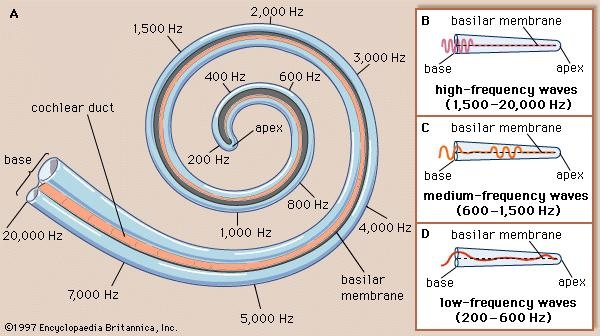
\includegraphics[width=0.8\textwidth]{./ucho.jpg}
    \caption{\label{fig:ucho} Schemat budowy ślimaka. Źródło \cite{enciclopidiabritanica}.}
\end{figure}
Znajdujące się na błonie podstawnej rzęski zagłębione, ustawione w rzędzie, wzdłuż ślimaka, zamieniają wychylenie błony na impulsy elektryczne wysyłane dalej przez nerw przedsionkowo-ślimakowy do mózgu. Ze względu na różnią sztywność błony podstawnej, narząd Cortiego w różny sposób interpretuje intensywność danej częstotliwości. Inne trzy równoległe rzędy rzęsek znajdujących dostarczają sprzężenia zwrotnego ze strony mózgu pozwalając na zwiększenie rozdzielczości przeprowadzonej analizy częstotliwościowej. Rzęski zewnętrzne pobudzane są głównie w rejonie największego ugięcia błony i poprzez to pobudzenie 'dostrajają' się do słyszanej częstotliwości.

Wykorzystanie wiedzy na temat budowy aparatu słuchowego przyniosło zdefiniowanie skal perceptualnych skal psychoakustycznych
\subsubsection{Skala Mela. \label{mel}}
Skala Mela jest nieliniową skalą częstotliwości powstałą poprzez subiektywne badanie psychoakustyczne. Relację pomiędzy skalą Mela a liniową skalą częstotliwości przybliża się zwykle wzorem:
\begin{equation}
  m = 2595\log_{10} \left( 1+ \frac{f}{700}\right),
\end{equation}
gdzie m oznacza wartość częstotliwości w Melach.

\begin{figure}[ht!]
  \centering
    \input{mel.pgf}
    \caption{\label{fig:mel} Relacja pomiędzy skalą Mela i liniową skalą częstotliwości.}
\end{figure}
\subsubsection{Skala Barka. \label{bark}}
Inną skalą perceptualną opartą na modelu ślimaka jako banku liniowych filtrów w skali częstotliwości jest skala Barka. Wyróżnia ona 24 pasma krytyczne. Zakłada się, że 1 bark odpowiada 100 melom, zaś funkcją przekształcenia ze skali liniowej jest:
\begin{equation}
  B = 13 \arctan \left( 0.00076\cdot f \right)+4.5\arctan\left(\frac{f}{7500}^2\right),
\end{equation}
gdzie B oznacza wartość w Barkach.

\subsubsection{Krzywe jednakowej głośności }
Ze względu na różną sztywność błony podstawnej (tak jak wskazano wczesniej w tym rozdziale) człowiek z inną intensywnością odbiera bodźce dźwiękowe związane z różnymi częstotliwościami. Z pomiarów subiektywnych na większej populacji wyznaczone zostały krzywe jednakowej głośności. Stosowane są one w niektórych technikach ekstrakcji cech (np. \ref{plp}) we wstępnym wzmocnieniu sygnału mowy.

\subsubsection{Układ nerwowy.}

Dziedzina rozpoznawania głosu jest szczególnie zainteresowana naturalną aparaturą w którą wyposażony jest człowiek dla zadania rozpoznawania mowy czy identyfikowania swoich rozmówców. Dotyczy to także całego obszaru metod rozpoznawania sygnałów akustycznych. Trend jest szczególnie widoczny związku z bardzo dynamicznym rozwojem dziedziny sztucznych sieci neuronowych i sztucznej inteligencji. Tak jak wspomniano wyżej, szereg metod związanych z rozkodowywaniem sygnału mowy - ekstrakcją cech - korzysta z wiedzy anatomicznej przy okazji konstrukcji algorytmów. Niestety w dziedzinie klasyfikacji mówców to podejście nie jest stosowane - prawdopodobnie ze względu na skromną wiedzę o tym jak funkcjonuje ludzki umysł. Wydaje się jednak, że można przywołać pewną wiedzę na temat tego jak człowiek interpretuje sygnał mowy poprzez wskazanie pewnych obszarów mózgu odpowiedzialnych za zadania związane z analizą mowy - a także połączenia pomiędzy nimi. Wraz z zastosowaniem rezonansu magnetycznego (MRI) neurologia poczyniła duże postępy i można mieć nadzieję na to, że w najbliższej przyszłości uzyskana wiedza pozwoli na udoskonalenie systemów rozpoznawania głosu.

\subsection{Klasyfikacja języka.}
\label{formant}
Na rysunku \ref{fig:spectrum} znajduje się przykładowe widmo pojedynczej ramki sygnału. Obszary koncentracji energii w dziedzinie częstotliwości nazywane są formantami. Analiza zmiany pozycji formantów pomiędzy kolejnymi fonemami okazuje się być bardzo ważna w zadaniu rozpoznawania mówców. 

\begin{figure}[ht!]
  \centering
    \input{spectrum.pgf}
    \caption{\label{fig:spectrum} Przykładowe spektrum pojedynczej ramki sygnału mowy.}
\end{figure}

\subsubsection{Fonetyka}
Fonetyka zajmuje się badaniem dźwięków produkowanych przez aparat mowy człowieka. Elementarnym dźwiękiem rozpatrywanym przez fonetykę jest głoska. Z punktu widzenia całej lingwistyki jest to najmniejszy segment mowy. Budowa i funkcjonalność narządu mowy determinują zakres produkowanych głosek. Fonetyka bada podstawowe dźwięki mowy bez rozróżniania ze względu na konkretny język czy znaczenie głoski.
Fonem jest najmniejszą jednostką mowy na podstawie której możliwa jest interpretacja jej znaczenia. To znaczy, że jest semantycznie istotna. Fonem rozpatruje się ze względu na znaczenie w konkretnym języku. Głoska może być realizacją fonemu. Dwie różne głoski mogą stanowić realizację tego samego fonemu - to znaczy nieść tę samą informację semantycznie. Zbiór takich głosek realizujących dany fonem nazywany jest alofonem.

Z punktu widzenia mechanizmów powstawania dźwięków w ludzkim narządzie mowy, można wyróżnić trzy z których zbudowany jest każdy emitowany dźwięk mowy. Składa się na nie:
- dźwięk rezonujący powstały w wibrującym źródle (np. drgające fałdy głosowe) i rezonujący w przestrzeni rezonansowej na którą składają się drogi oddechowe znajdującą się powyżej krtani,
- dźwięk powstały przez nielaminarny przepływ powietrza,
- dźwięk impulsowy powstały przez energiczne wypuszczenie powietrza z układu oddechowego.

\section{Ekstrakcja cech sygnału mowy.}

\label{featureextraction}
\subsection{Przegląd.}
Celem ekstrakcji cech z sygnału mowy (\textit{ang. feature extraction}) jest uzyskanie zbioru cech charakteryzujących sygnał ludzkiej mowy za pomocą technik cyfrowego przetwarzania sygnału. Jednocześnie jest to zamiana sygnału w którym zawarta jest redundantna informacja na sygnał o niskiej zawartości informacji znaczących dla problemu rozpoznawania mówcy/mowy. 

%todo przeredagowac bo to nie ma sensu xd nie rozumiem tych reduckji
W ogólności system produkcji mowy człowieka można przedstawić jako układ regulacji automatyki z kontrolerem reprezentującym układ nerwowy wraz z kontrolowaną przezeń motoryką aparatu mowy. Sygnał sterujący kontrolera powoduje pobudzenie układu charakterystyk sygnału mowy charakteryzowany przez budowę dróg głosowych. Dopiero wyjściem tego ostatniego jest akustyczny sygnał mowy. Podczas gdy problem rozpoznawania mowy próbuje wyeliminować wpływ na formułowany model postaci układu charakterystyk głosowych, tak rozpoznawanie niezależne od tekstu próbuje ustalić model charakterystyk głosowych bez względu na postać układu kontrolera. Ponieważ oba rozpatrywane modele są mocno nieliniowe najtrudniejszym zadaniem w rozpoznawaniu mówcy jest ich rozdzielenie. Z tego właśnie powodu problem ze znanym wypowiadanym tekstem jest o wiele prostszym zagadnieniem od problemu rozpoznawania mówcy niezależnego od wypowiadanego tekstu. W tym pierwszym przypadku dokonujemy redukcji do tylko znanych pobudzeń oraz konkretyzować model kontrolera $G_c$. %TODO

Przedstawione w tym podrozdziale techniki ekstrakcji cech okazują się równie przydatne i powszechnie stosowane zarówna dla technik rozpoznawania mówcy jak i rozpoznawania mowy. Najpopularniejszą obecnie stosowaną metodą ekstrakcji cech z sygnału mowy jest współczynnikami cepstrum w dziedzinie częstotliwości Mela -  MFCC (\textit{ang. Mel-Frequency Cepstral Coeficcients}). 

Ważnym elementem toru przetwarzania systemu są również elementy związane z zaszumieniem sygnału mowy, przetwornikiem elektroakustycznym oraz procesem dyskretyzowania elektrycznego sygnału mowy przez przetwornik analogowo-cyfrowy. Jednak ze względu na prostotę te zagadnienia zostaną omówione oddzielnie od problemu ekstrakcji cech.

\subsection{MFCC.}
\label{mfcc}

Ekstrakcja cech za pomocą współczynników cepstrum w dziedzinie częstotliwości Mela składa się z dwóch głównych etapów: uzyskania współczynników mocy w dziedzinie częstotliwości Mela na podstawie estymacji widma mocy sygnału mowy (\textit{freqency warping}) oraz obliczenia współczynników cepstrum na podstawie uzyskanych wcześniej współczynników mocy w skali Mela. Wynikiem przeprowadzonej operacji jest uzyskanie wektora cech $x_j$ dla numeru ramki $j$.

\subsubsection{DSTFT - dyskretna krótkookresowa transformata Fouriera}
Dyskretna krótkookresowa transformata Fouriera (DSTFT - \textit{ang. Discrete Short-time Fourier Transform}) jest dyskretną wersją ciągłej transformaty Fouriera (STFT - \textit{ang. Short-time Fourier Transform} dla sygnału próbkowanego w czasie oraz dyskretnego w dziedzinie częstotliwości. Jest to metoda analizy czasowo-częstotliwościowej, przeprowadzając oparację dyskretnej transformaty Fouriera (DFT - \textit{ang. Discrete Fourier Transform}) na ramkach sygnału dla których możemy założyć jego lokalną stacjonarność. Relacja pomiędzy STFT, a DSTFT jest relacją analogiczną do relacji ciągłej transformaty Fouriera, a DFT.  Estymacja widma za pomocą metody DSTFT jest podstawą techniki ekstrakcji cech MFCC.

\subsubsection{Podział sygnału na ramki.}
Ze względu na własność quasi-stacjonarności sygnału mowy, aby wydobyć informację dotyczącą wypowiadanej głoski konieczne jest rozdzielenie sygnału na ramki.
Liczbę próbek dla pojedynczej ramki wybiera się ze względu na konieczność uzyskania lokalnej stacjonarności - w taki sposób aby było możliwe zbadanie charakterystyki częstotliwości pojedynczej głoski. Średnia długość głoski to 80 ms. Jednak trzeba mieć na względzie, że samogłoski trwają długo w stosunku do przerw pomiędzy (trwających zwykle ok. 5 ms). Zatem aby móc uchwycić krótsze głoski oraz przerwy zwykle ustala się długość ramki na 20 do 30 ms. Jednocześnie długość ramki w ilości próbek jest funkcją częstotliwości próbkowania. Do przedstawionych założeń dochodzi zwykle warunek dotyczący użycia algorytmu szybkiej transformaty Fouriera (FFT - \textit{ang. Fast Fourier Transform}) wymagającej aby sygnał był długości potęgi dwójki. W przypadku pierwszej oraz ostatniej ramki stosowana jest technika uzupełniania zerami w przypadku braku próbek do zapełnienia całej ramki.

\subsubsection{Aplikacja okna na ramki.}
W wykorzystywanej technice DSTFT stosowane są zazwyczaj okna inne niż okno prostokątne o takiej samej długości jak ramki w celu zredukowania przecieku widma. Zastosowanie okna czasowego odbywa się poprzez przemnożenie wartości próbek ramki przez wartości okna w następujący sposób:
\begin{equation}
  h_i = w_i \cdot x_i, \quad i \in {1,...,N}
\end{equation}
gdzie $x_i$ oznacza i-tą próbkę sygnału, $h_i$ - zmodyfikowaną wartość próbki użytej dla wyznaczania współczynników DFT, $w_i$ - i-tą wartości funkcji okna, $N$ ilość próbek w ramce. 

Najpopularniejszymi oknami stosowanymi w tym przypadku są okna czasowe Hanna, Hamminga oraz okna Gaussowskie \cite{fosr}.

\subsubsection{Estymacja widma.}
\label{stft}
Po zaaplikowaniu okien czasowych dla kolejnych ramek sygnału, kolejnym etapem procedury obliczania współczynników MFCC jest znalezienie widma ramki za pomocą dyskretnej transformaty fouriera (DFT). Kolejne współczynniki uzyskanego widma zdefiniowane są następująco:
\begin{equation}
  H_k = \sum^{N-1}_{n=0} h_n exp(\frac{-2\pi kn}{N} )
\end{equation}
W omawianej metodzie korzysta się jedynie z informacji o amplitudzie uzyskanego widma. Kolejne współczynniki widma amplitudowego zdefiniowane są w następujący sposób:
\begin{equation}
  M_k = |H_k| = \sqrt{H_k^2}
\end{equation}

\subsubsection{Przejście do dziedziny częstotliwości Mela.}
Przejście do dziedziny częstotliwości Mela (\textit{ang. frequency warping}) uzasadnione jest nieliniową percepcją układu słuchowego człowieka. Ponieważ procedura DFT produkuje liniowe widmo w dziedzinie widmo częstotliwościowe, dokonywana jest jego transformacja do dziedziny częstotliwości Mela. Jest to proces imitujący cechę sygnału akustycznego - wysokości tonu.
Rozpatrywana operacja polega na zastosowaniu banku filtrów trójkątnych na uzyskanych amplitudach widma kHz:
\begin{equation}
  \tilde{H}_j = \sum_{k=1}^{K} H_k \cdot F_k, \quad k \in {1...N}, \quad  j \in {1...M}
\end{equation}
gdzie $\tilde{H}_j$ oznacza j-ty współczynnik amplitudy widma w dziedzinie częstotliwości Mela, $F_k$, zaś $M$ oznacza ilość filtrów.
W wyniku tej operacji otrzymuje się wektor współczynników częstotliwości w skali Mela o długości równej ilości użytych filtrów. Najczęściej stosowanym filtrem jest okno trójkątne zdefiniowane w dziedzinie częstotliwości. Każdy kolejny filtr zaczyna się w środku pasma wcześniejszego. Ponieważ przetwarzany jest sygnał składający się z próbek o wartościach rzeczywistych, pokryte pasmo częstotliwości zawiera próbki od 0-wej do próbki o oznaczonej numerem N/2. Ilość filtrów oraz ich rozmieszczenie w dziedzinie częstotliwości ustalane są na jeden z kilku sposobów.
Pierwszym sposobem jest skorzystanie z 24 obszarów krytycznych zdefiniowanych w skali Barka. Każdy filtr ma niezerowe wartości w zakresie częstotliwości od k-1 częstotliwości krytycznej, aż do k+1 częstotliwości krytycznej. Maksimum zaś przypada na k-tą częstotliwość krytyczną.
Drugim i najpopularniejszym podejściem jest zastosowanie ustalonej ilości filtrów i rozmieszczenie ich równomiernie w dziedzinie częstotliwości mela.

\begin{figure}
  \centering
    \input{melfb.pgf}
    \label{melfb}
    \caption{Przykładowe 24 trójkątne filtry dla sygnału o częstotliwości próbkowania \textit{fs=12500 Hz.}}
\end{figure}

Stosowane są również filtry trapezowe oraz kosinusowe, a także zmianę wzmocnienia filtrów ze względu na psychoakustyczną krzywą jednakowej głośności. 

\subsubsection{Uzyskanie współczynników głośności.}
Wartości otrzymane w procesie przejścia do dziedziny częstotliwości Mela z prążków reprezentujących widmową gęstość mocy sygnału mogą reprezentować natężenie dźwięku w danym momencie czasu. Ponieważ zadaniem ekstrakcji cech przy pomocy współczynników MFCC jest mimika ludzkiego układu percepcji konieczne jest przekształcenie wartości reprezentujących energię na głośność (\textit{ang. magnitude warping}). Zgodnie z przedstawioną definicją \ref{glosnosc} \textit{głośność} jest funkcją zarówno \textit{wysokości tonu} oraz natężenia dźwięku $ I $. Relację z \textit{wysokością tonu} imituje się za pomocą etapu \textit{equalizacji} sygnału. Zatem pozostaje jedynie zdefiniować współczynniki głośności $ C_k $ \cite{fosr} dla każdej ramki sygnału:
\begin{equation}
  \tilde{C_k} = 10 \cdot \left( \frac{|\tilde{H_k}|^2}{I_0} \right) 
\end{equation}

Ponieważ normalizacja współczynników w postaci odniesienia wartości współczynników widma mocy do natężenia odniesienia $I_0$ nie wpływa na efekt identyfikacji mówcy dlatego w praktyce stosuje się dla wygody postać (szczególnie ze względu na pokrywanie się tych wartości z elementami przetwarzanymi w procedurze otrzymywanie cepstrum sygnału \ref{cepstrum}):
\begin{equation}
  C_k = log \left(|\tilde{H_k}|^2 \right)
\end{equation}
Przy użyciu tych współczynników otrzymuje się cepstrum sygnału.

\subsubsection{Cepstrum.}
\label{cepstrum}

Funkcja cepstrum mocy dla ciągłego przekształcenia Fouriera zdefiniowana jest następująco \cite{fosr}:
\begin{equation}
    \tilde{h_{pc}} = \left[\frac{1}{2\pi}\int_{-\pi}^{\pi}log\left(| H(\omega)  |^2\right)e^{i \omega t}\right]^2
\end{equation}
gdzie $ |H(\omega)|^2 $ oznacza funkcję widma gęstości mocy sygnału oryginalnego. Jest to odwrotne przekształcenie Fouriera zastosowane na logarytmie funkcji gęstości mocy sygnału.
   
Pojęcie cepstrum pierwotnie zostało wprowadzone do badań nad echem sygnałów akustycznych \cite{hdsp}. Taki sygnał opisywany jest przez wyrażenie 
\begin{equation}
     x(t) = s(t) + \alpha s(t - \tau) 
\end{equation} 
gdzie $ \alpha $ jest współczynnikiem osłabienia sygnału echa przesuniętego w czasie o $ \tau $ względem sygnału oryginalnego. Reprezentacja częstotliwościowa zaś przyjmuje w takim wypadku postać 
\begin{equation}
    |S(f)|^2\left[ 1+ \alpha^2+2\alpha cos(2\pi f\tau)\right].
\end{equation}
Jak widać z tej postaci, widmo sygnału oryginalnego $S(f)$ modulowane jest przez zmienny w częstotliwości komponent $[1 + \alpha^2 + 2\alpha cos(2\pi f \tau)]$. Znajomość tego w jaki sposób modulowana jest obwiednia widma pozwala na określenie współczynników $\alpha$  oraz $\tau$ definiujących sygnał echa. Ponieważ problem taki jest doskonale opisany w dziedzinie czasu przy analizie sygnałów zmodulowanych, narzucającym się rozwiązniem jest skorzystanie z tych znanych już technik. Korzystając z własności logarytmu możliwe jest rozdzielenie dwóch komponentów - zamianę mnożenia na dodawanie, a poprzez zastosowanie odwrotnego przekształcenia Fouriera otrzymuje się sumę dwóch funckji w dziedzinie tzw. "quefrency": 
\begin{equation}
    \begin{split}
    \mathcal{F}^{-1}\{log(X(f))\} =   \mathcal{F}^{-1}\{log(S(f))\} + \mathcal{F}^{-1}\{log(1+\alpha^2)\} + \\ + \mathcal{F}^{-1}\{log(1+\frac{2a}{1+a^2} cos(\omega \tau))\}.
    \end{split}
\end{equation}
Ostatni składnik powyższej sumy objawia się w postaci widocznego w cepstrum skupionego impulsu którego położenie w skali cepstrum określa przesunięcie $\tau$ zaś jego amplituda jest związana z czynnikiem osłabienia $\alpha$. 

Okazuje się, że problem wykrycia wysokości tonu (\textit{ang. pitch detection}) sygnału mowy jest podobny do problemu analizy echa sygnału akustycznego. Zaproponowana została więc wersja wykorzystująca cepstrum dla analizy STDFT\cite{noll}. Prosty model produkcji sygnału mowy zakłada, że ten jest wynikiem splotu odpowiedzi impulsowej dróg głosowych $h_1$ oraz quasi-okresowym sygnałem impulsowym $h_2$ (\textit{ang. quasi-periodic pulse train}) - wymuszeniem produkowanym przez głośnię:
\begin{equation}
    h(t) = h_1(t)*h_2(t)
\end{equation}
Z własności ciągłego przekształcenia Fouriera wynika, że powyższe równanie w dziedzinie częstotliwości przybiera postać iloczynu transformat $H_1(\omega) \cdot H_2(\omega)$. W dziedzinie cepstrum rozdziela się natomiast na sumę składników:
\begin{equation}
    \tilde{h}(t) = log(H_1(\omega)) + log(H_2(\omega))
\end{equation}

Poprzez obliczenie cepstrum sygnału mowy otrzymujemy zatem rozdzielenie komponentów pochodzących od funkcji $h_1(t)$ i $h_2(t)$. Proces ten nazywany jest również dekonwolucją (\textit{homomorphic deconvolution})\cite{hdsp} i  zobrazowany jest na rysunku \ref{fig:e_cepstrum}. Niskie współczynniki cepstrum opisują charakterystykę aparatu głosowego, zaś widoczne w okolicach próbki 77 i 150 piki, stanowią harmoniczne w dziedzinie cepstrum (\textit{ang. rahmonics}) i świadczą o okresie sygnału wymuszenia głośni ($h_2$), którą można odczytać z pierwszego wykresu jako odległość w próbkach pomiędzy najwyższymi szczytami - 77 próbek.

\begin{figure}
  \centering
  \begin{minipage}{.5\textwidth}
    \centering
    \input{e_vowel.pgf}
  \end{minipage}%
  \begin{minipage}{.5\textwidth}
    \centering
    \input{e_cepstrum.pgf}
  \end{minipage}
  \caption{Ramka sygnału wypowiadanej samogłoski 'i' oraz jej cepstrum.}
  \label{fig:e_cepstrum}
\end{figure}

Należy zwrócić uwagę, że wykorzystywany w tej metodzie jest logarytm z liczb rzeczywistych oraz współczynniki mocy widma. Spowodowane jest to, że podczas procesu rozpoznawania mówcy nie interesuje nas rekonstrukcja sygnału, anie nie korzysta się z informacji zachowanej w fazie sygnału. Z tego też powodu klasycznie w ostatnim etapie obliczania współczynników MFCC zamiast odwrotnej dyskretnej transformaty Fouriera (IDFT) stosuje się dyskretną transformację kosinusową (DCT). Kolejną korzyścią jest otrzymanie w wyniku przeprowadzenia tej transformacji współczynników będącymi liczbami rzeczywistymi. W tej pracy korzysta się z następującej definicji dyskretnej transformaty kosinusowej:
\begin{equation}
  \label{dct}
    H_k = \sum_{n=0}^{N-1} h_ncos\left(\frac{\pi (2n+1)k}{2N}\right)
\end{equation}
gdzie
\begin{equation}
    a_k = 
    \begin{cases}
        1/N \quad \text{dla}\quad k=0 \\
        2/N \quad \forall \quad k>0.
    \end{cases}
\end{equation}

Uzyskane współczynniki MFCC noszą nazwę wektora akustycznego (\textit{ang. acoustic vector}) reprezentującą cechy pojedynczej ramki i są w procesie weryfikacji mówcy dalej wykorzystywane w tzw. procesie dopasowywania cech opisanym w sekcji \ref{featurematching}.

W wektorze cech zwykle stosuje się od 12 do 15 najniższych współczynników uzyskanych z DCT. Zwykle uzupełnia się go dodatkowymi współczynnikami $\Delta$ oraz $\Delta^2$ zawierające dodatkową informację o dynamice sygnału. 

\subsubsection{Współczynniki Delta cepstrum oraz Delta-Delta cepstrum}

  Tak jak opisano dalej w tej pracy w \ref{otherfeatures}, duże znaczenie w procesie rozpoznawania mówcy ma informacja temporalna zawarta w sygnale mowy - związana z dynamiką zmian współczynników kolejnych ramek wektorów cech. Najpopularniejszą metodą na dodanie informacji tego rodzaju jest dołączenie do wektora cech MFCC współczynników \textit{Delta} - $\Delta$ oraz \textit{Delta-Delta} - $\Delta^2$ które kolejno reprezentują pierwszą i drugą pochodną dyskretną dla kolejnych ramek sygnału. Okazuje się, że dodanie wspomnianych współczynników daje znaczącą poprawę procesu rozpoznawania, szczególnie w systemach rozpoznawania mówcy z hasłem lub zależnego od wypowiadanego tekstu \cite{delta}. Najczęściej, stosuje się następującą formułę do obliczenia cech delta cepstrum:
\begin{equation}
  \Delta_{t, k} = \frac{\sum^N_{n=1} n(c_{t+n,k} - c_{t-n,k})}{2\sum^N_{n=1} n^2} 
\end{equation}
gdzie $N$ przyjmuje typową wartość 2, $C_{t,k}$ oznacza współczynnik cepstrum dla ramki $t$ i numerze współczynnika w ramce $k$. Współczynniki Delta-Delta obliczane są w ten sam sposób za wyjątkiem użycia współczynników Delta w miejsce współczynników cepstrum:
\begin{equation}
  \Delta^2_{t, k} = \frac{\sum^N_{n=1} n(\Delta_{t+n,k} - \Delta_{t-n,k})}{2\sum^N_{n=1} n^2} 
\end{equation}
Do wektora cech MFCC dodaje się zwykle taką samą ilość współczynników $\Delta$ oraz $\Delta^2$ co współczynników cepstrum $c_{k}$. W systemach rozpoznawania mówcy bez znajomości wypowiadanego tekstu proponuje się ograniczyć ilość współczynników delta w stosunku do współczynników cepstrum i współczynników delta-delta w stosunku do współczynników delta \cite{fosr}.

\subsection{LPCC}
\label{LPCC}

Współczynniki liniowego kodowania predykcyjnego cepstrum - LPCC (\textit{ang. linear predicting ceptstral coding}) są alternatywną metodą ekstrakcji cech z sygnału mowy. Jest to synteza metody kodowania LPC wraz z zastosowaniem współczynników cepstrum. Liniowe kodowanie predykcyjne (LPC) jest techniką opartą na zastosowaniu modeli autoregresyjnych (AR). Główną różnicą w stosunku do techniki MFCC jest więc sposób aproksymacji widmowej gęstości mocy przy pomocy współczynników $|H_k(\omega)|^2$. Kroki wstępnego przetwarzania poprzedzające estymację, łącznie z aplikacją na ramkę okna czasowego, są identyczne jak w przypadku procedury obliczania współczynników MFCC. Zamiast posługiwać się dyskretnym przekształceniem Fouriera (DFT), korzysta się z modelu autoregresyjnego, kształtując widmo przy pomocy transmitancji $H(z)$ posiadającej same bieguny (\textit{ang. all-pole}) i jednym zerem w punkcie $z =0$:
\begin{equation}
  \label{transar}
  \tilde{H}(z) = \frac{\tilde{G}}{1-\sum_{k=1}^{p} a_k z^{-k}}
\end{equation}
gdzie $ a_k = \frac{\alpha_k}{\alpha_0} $, $\tilde{G} = \frac{1}{\alpha_0}$, a współczynniki $\alpha_0,...,\alpha_p$ oznaczają współczynniki modelu AR, nazywane również w rozpatrywanym przypadku jako współczynniki predykcji - PC (\textit{ang. predictor coefficients}).

W dziedzinie czasu modele liniowej predykcji (LP) określają zależność próbki sygnału $s_n$ poprzez liniową kombinację wcześniejszych p próbek przeskalowanych przez współczynniki predykcji - PC:
\begin{equation}
  s_n = - \sum_{k=1}^{p}a_k\cdot s_{n-k}+\tilde{G}\cdot u_n
\end{equation}
W metodach liniowej predykcji zazwyczaj ignoruje się wartość $u_n$ oznaczającą obecną próbkę wejściową - w przypadku mowy oznaczającą sygnał tonu krtaniowego. W ten sposób otrzymuje się wektor współczynników $a_1,...,a_n$ modelujących danego mówcę. Popularną metodą estymacji tych wartości jest minimalizowanie wartości błędu średniokwadratowego wartości resztowych (rezydua):
\begin{equation}
  V = \sum_{n} e_n^2 = \sum_n \left\{ s_n + \sum_{k=1}^p \alpha_k \cdot s_{n-k} \right\}.
\end{equation}
Kryterium minimalizacji
\begin{equation}
  \frac{\delta E}{\delta \alpha_i} = 0, \quad i=1,..,p
\end{equation}
daje w wyniku zależność:
\begin{equation}
  \label{yweq}
  \sum_{k=1}^{p} a+k \cdot \sum_n s_{n-k} s_{n-i} = - \sum_n s_n s_{n-i}, \quad  i=1,...,p.
\end{equation}
Lewa suma $ \sum_n s_{n-k} s_{n-i} $ jest funkcja autokorelacji o opóźnieniu $ \tau = n-k $, czyli $ r(|n-k|) $, zaś analogicznie prawa jest funkcją autokorelacji o opóźnieniu $ \tau = n $ tzn. $ r(n)$, gdzie w obu przypadkach $i=1,...,p$.
Układ tych równań nazywany jest równaniami Yule'a-Walkera (\textit{Yule-Walker Equations}). Otrzymana z tych równań macierz autokorelacji $ \bm{R} $ przyjmuje postać macierzy Toeplitza - posiada te same wartości na poszczególnych przekątnych. Rozwiązanie problemu minimalizacji przedstawia się jako:
\begin{equation}
  \bm{\alpha} = \bm{R^{-1}} \bm{r},
\end{equation}
gdzie wektor $ \bm{r}$ jest wektorem kolumnowym prawych sum równań \ref{yweq} tzn. autokorelacji $ r(n)$, zaś wektor $ \bm{\alpha} $ wektorem kolumnowym współczynników $\alpha_1,...,\alpha_n$. Wspomniana własność macierzy $\bm{R}$ jako macierzy Toeplitza w dużym stopniu upraszcza procedurę odwracania macierzy poprzez zastosowanie rekursywnego algorytmu \textit{Levinsona-Durbina}\cite{durbin}. Możliwy do zastosowania algorytm Shura\cite{shur} pozwala przyspieszyć obliczenia poprzez paralelizację. Obliczone wartości $\alpha_i$ reprezentują współczynniki LPC. Wraz z wartością:
\begin{equation}
  \tilde{G} = r(0) - \sum_{i=1}^{p} a_i r(i)
\end{equation}
umożliwiając aproksymację funkcji gęstości widma przy pomocy równania \ref{transar}.

\subsubsection{Obliczanie współczynników LPCC}
W praktyce \cite{fosr} jako wektory cech najczęściej używa się współczynników cepstrum obliczonych przy pomocy uzyskanych współczynników LPC. Rekursywny algorytm zaproponowany przez Rabinera i Juanga \cite{rabinerjuangfosr60} oblicza współczynniki cepstrum w następujący sposób:
\begin{enumerate}
    \centering
  \item $c_0 = log(\tilde{G}^2)$,
  \item $c_d = \alpha_d + \sum_{i=1}^{d-1} c_i a_{d-i} \quad \textrm{\textbf{dla}} \quad 1\leq d \leq p$
  \item $c_d = \sum_{i=1}d + \sum_{i=1}^{d-1} c_i a_{d-i} \quad \textrm{\textbf{dla}} \quad d > p$
\end{enumerate}

Rekomendowana ilość $p$ dla obliczania współczynników LPCC powyższym sposobem to zakres od 8 do 16 \cite{fosr}. Najczęściej stosuje się liczbę 8 do 20 elementów w wektorze cech. 
\subsection{Inne metody ekstrakcji cech.}
Najczęściej stosowanymi metodami ekstrakcji cech są następujące: MFCC, LPCC, LSF, PLP \cite{overview}. Dwie pierwsze zostały omówione wcześniej bardziej szczegółowo. W tym zaś podrozdziale pokrótce zostały omówione dwie kolejne oraz inne wybrane metody, które pojawiają się w literaturze fachowej oraz artykułach użytych jako źródła w tej pracy jako te metody które mogą mieć znaczenie w dalszym rozwoju omawianej dziedziny.
\subsubsection{Metody bazujące na LP}
Istnieje szereg innych metod opartych na współczynnikach LP. Zwykle cechuje je nieliniowa transformacja dziedziny czasu/częstotliwości oraz amplitud współczynników mocy widma, która na celu ma przybliżyć sposób funkcjonowania percepcji ludzkiego aparatu słuchowego w konstruowanym systemie. 
\begin{itemize}
  \item{PARCORs (\textit{ang. partial correlation coefficients})} - \textit{współczynniki częściowej korelacji} są współczynnikami cech $\kappa_k$ interpretowanymi jako wartość reprezentującą nieredundantną informację o autokorelacji\cite{fosr}. Wielkości te są obliczane jako wartości pośrednie w algorytmie obliczania współczynników LPC we wcześniej wspomnianym (\ref{LPCC}) algorytmie Levinsona-Durbina. Współczynniki te również mają interpretację fizyczną jako modelujące wartości współczynników odbicia w modelu traktu głosowego jako cylindrów o różnych średnicach przez które przepływa strumień powietrza z płuc\cite{flanganfosr21}. Z tego też powodu nazywane są także \textit{współczynnikami odbicia} (\textit{ang. reflection coefficients}).

  \item{LAR \textit{ang. Log Area Ratios}} - wielkości wynikające z modelu cylindrów tak jak w metodzie PARCORs. Współczynniki $ g_i $ otrzymuje się jako stosunki logarytmów średnic kolejnych cylindrów modelu. Tak obliczone współczynniki cechują się bardziej równomierną wrażliwością w dziedzinie częstotliwości niż współczynniki odbicia\cite{campbell}.

  \item{PLP (\textit{ang. Perceptual Linear Predictive analysis}\label{plp}} - metoda ekstrakcji cech oparta na współczynnikach predykcji liniowej (LP) inspirująca się metodą MFCC. Zamiast zastosowania skali mela, w tej metodzie używa się skali Barka \ref{bark}, stosuje się zmodyfikowaną preemfazę ze względu na krzywą jednakowej głośności (\textit{ang. equal-loudness pre-emphasis}) \ref{loudness} oraz dokonuje się transformacji widma amplitudowego poprzez podniesienie wartości do potęgi $\frac{1}{3}$ co powoduje wygładzenie widma - zmniejszeniem dynamiki - i jest nazywana konwersją natężenia dźwięku do poziomu głośności (\textit{ang. Intensity to Louadness Conversion}) \cite{hoening}. Po tych etapach, z tak przekształconego widma uzyskiwane są współczynniki predykcji liniowej (model AR). Tak jak w metodzie MFCC także i tutaj używa się procedury DFT i IDFT. Współczynniki cepstrum uzyskiwane są tak jak w metodzie LPCC, np. przy wykorzystaniu metody Levinsona-Durbina. Na rysunku \ref{plp} przedstawiono etapy analizy PLP tak jak w pracy źródłowej \cite{fosr30hermansky}.

\begin{figure}[ht!]
  \centering
    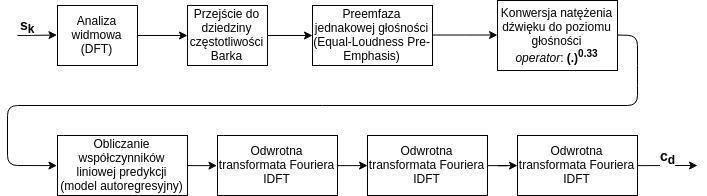
\includegraphics[width=1.1\textwidth]{plp.png}
    \caption{\label{plp} Etapy analizy PLP.}
\end{figure}

\item{LSF (\textit{ang. line spectral frequencies} lub LSP (\textit{ang. line spectral pairs}))} - metody reprezentacji sygnału mowy w których zaproponowana jest alternatywna postać mianownika transmitancji z \ref{transar}. Oznaczając mianownik jako $A(z)$ przyjmowana jest reprezentacja:
  \begin{equation}
  \begin{gathered}
    A(z) = \frac{1}{2} [P(z) + Q(z)] \\
    P(z) = A(z) + z^{p+1} A(Z^{-1}) \\
    Q(z) = A(z) - z^{p+1} A(Z^{-1}). 
  \end{gathered}
  \end{equation}
    gdzie wielomian $P(z)$ jest interpretowany fizycznie jako odpowiadający odpowiedzi impulsowej dróg głosowych przy głośni zamkniętej zaś wielomian $Q(z)$ przy otwartej. Pierwiastki wielomianów $P$ i $Q$ leżą na okręgu jednostkowym na płaszczyźnie zespolonej $z$. Techinka ta jest nazywana \textit{ang. reverse-filtering}. 
\end{itemize}

\subsubsection{Metody wykorzystujące transformację falkową.}

Tak jak wcześniej opisano w rozważaniach o krótko-czasowej transformacie Fouriera (STFT) \ref{stft}, niestacjonarny sygnał mowy możemy analizować metodami czasowo-częstotliwościowymi z odpowiednio małym oknem dobranym na podstawie czasu trwania pojedynczych głosek. Segmentacja sygnału na takie ramki pozwalała zastosować metody estymacji widma dla sygnały stacjonarnego. Metody estymacji widma z zastosowaniem modeli autoregresyjnych (AR) również przyjmują, że działają na sygnale stacjonarnym. Transformacja falkowa dostarcza szeregu ortogonalnych funkcji jądra dla uogólnionego szeregu Fouriera. Wspomniane funkcje powstają poprzez rozciąganie i przemieszczanie funkcji matki dla danej transformacji falkowej. Warto zwrócić uwagę na to, że transformacja Gabora, będącą transformacją falkową z funkcją matką równą iloczynowi jądra transformaty Fouriera $ exp(-2\pi j f \tau)$ oraz funkcją Gaussowską $ exp(-\pi(\tau-t)^2) $ stanowi przypadek krótko-czasowej transformaty Fouriera (STFT) dla której użyto okna Gaussowkiego. Zatem widać, że istnieje pole do zastosowania analizy czasowo-częstotliwościowej w postaci transformacji falkowej w miejsce STFT czy estymacji za pomocą modeli autoregresyjnych. Odpowiednikiem dyskretnej transformaty Fouriera (DFT) jest dyskretna transformata falkowa (DWT -\textit{ang. discrete wavelet transform}).
\begin{enumerate}
  \item{MFCWC - \textit{Mel-Frequency Discrete Wavelet Coefficients}} - technika oparta na generacji współczynników MFCC - jest praktycznie identyczna w kolejnych krokach za wyjątkiem wykorzystania transformaty cosinusowej (DCT) w zamian za użycie dyskretnej transformaty falkowej (DWT). Okazuje się, że zastosowanie DWT przyczynia się do polepszenia rezultatów w 'agresywnie' hałaśliwym środowisku\cite{fosr}.
  \item{WOCOR - \textit{Wavelet Octave Coefficients Of Residues}} - jest wektorem cech wyekstrahowanych za pomocą transformacji falkowej z funkcją matką związaną z tonem wypowiadanej głoski, co wiąże się z rozmiarem analizowanej ramki. Jest to metoda oparta na współczynnikach liniowej predykcji (LP) rezyduł sygnału w ramce. Rozważana technika jest efektywna w użytku z sygnałem mowy zawierającym języki oparte na intonacji (\textit{ang. pitch-based}) takie jak dialekty języka Chińskiego  - Mandaryński czy Kantoński \cite{fosr}.
\end{enumerate}

\subsubsection{Inne metody ekstrakcji cech.}
\label{otherfeatures}

Istnieje szereg metod bazujących na przekształceniu dziedziny czy wartości współczynników funkcji gęstości widmowej sygnału za pomocą banku filtrów o różnych właściwościach. Zamiast banku filtrów mela (MFCC) lub Barka (PLP) konstruowane są filtry bazujące na innych, bardziej specyficznych modelach ludzkiego narządu słuchu \cite{fosr}.

Większość opisanych wcześniej techniki ekstrakcji cech z sygnału mowy są metodami określanymi jako widmowe i krótko-czasowe (\textit{ang. Short-Term Spectral Features})\ref{overview} z ramkami sygnału o długości od 20 do 30 ms.

Cechy temporalno-widmowych(\textit{ang. Spectro-Temporal Features})\cite{overview} są zbiorem wielkości dostarczających informacji na temat tożsamości mówcy zawartej w przejściach pomiędzy formantami (\ref{formant}) czy modulacją amplitudy współczynników widma w czasie. Jednym ze sposobów na uzyskanie tego typu informacji jest zastosowanie opisanych wcześniej współczynników Delta ($\Delta$) i Delta-Delta ($\Delta^2$) dla cech MFCC \ref{delta}. Innymi skutecznymi technikami jest użycie współczynników regresji liniowej  czy wartościami aproksymacji wielomianami punktów dla kolejnych kilku wektorów cech (zwykle 2 lub 3) \cite{multidsp}. Nowszymi rozwiązaniami jest badanie wolnych modulacji amplitudy i częstotliwości w ramkach zawierających po ok 10wektorów cech, jak np. w metodzie TDCT (\textit{Temporal Discrete Cosine Transform}) [modulacja amplitud].

Istnieją również cechy wysokiego poziomu, takie jak cechy prozodyczne (\textit{ang. prosodic features}) które mogą identyfikować mówcę za pomocą rytmu, akcentu czy intonacji wypowiedzi. Opisywane w literaturze są również takie zestawy cech które operą nie na charakterystykach takich związanych ze stylem wypowiedzi czy zasobem słownictwa\cite{overview}.
\section{Metody klasyfikacji sygnału mowy. Modelowanie mówcy.}
\label{featurematching}

Procesy rozpoznawania mówcy, a w szczególności weryfikacji mówcy są podklasą szerszego zagadnienia znanego z techniki jako dopasowania wzorca (\textit{ang. pattern matching}). W ogólności celem przeprowadzonego zadania dopasowania wzorca jest określenie czy w dostarczonej na wejściu systemu sekwencji danych można znaleźć pewien znany wzorzec oraz określenie ilościowej relacji stopnia podobieństwa. W rozpatrywanym w tej pracy zadaniu weryfikacji mówcy oczekuje się, że element systemu odpowiedzialny za proces dopasowania wzorca zwróci wynik reprezentujący miarę podobieństwa wejściowego wektora cech do weryfikowanego modelu mówcy. Takie modele mówcy powstają z wektorów akustycznych dostarczonych jako zestaw danych uczących. W praktycznym systemie weryfikacji mówcy tak skonstruowane modele przechowywane są w postaci zaszyfrowanych danych. Następnie używane są do podjęcia decyzji o tym czy podający się za weryfikowaną osobę otrzyma dostęp do chronionych zasobów.

Obecnie dla etapu dopasowania wzorca - w klasycznym podejściu - stosowane są metody\cite{campbell} \cite{overview}: ukryte modele Markowa (\textit{ang. HMM - hidden Markov model}, dynamiczne dopasowanie czasowe (\textit{ang. DTW - Dynamic Time Warping}), kwantyzacja wektorów (\textit{VQ - vector quantization}, mikstury Gaussowskie (\textit{GMM - Gaussian mixture model}), (\textit{SVM - support vector machine}) oraz sztuczne sieci neuronowe (\textit{ANN - artificial neural network}).

Wyróżnia się dwie grupy technik dopasowania wzorca: techniki deterministyczne (\textit{ang. template models}) oraz techniki probabilistyczne (\textit{probabilistic models})\cite{campbell}.

W grupie technik deterministycznych, w trakcie trwania fazy modelowania (trenowania), z wprowadzonych danych uczących generowane są wektory wzorcowe w sposób zależny od wybranego algorytmu - mogą to być z góry narzucone wartości, uśrednione wartości wektorów  czyli centroidy (\textit{ang. centroids}), np:
\begin{equation}
  \tilde{x} = \mu = \frac{1}{N}\sum_{i=1}^{N}x_i.
  \label{centroid}
\end{equation}
lub takie wzorcowe wektory mogą być ustalone w inny sposób. W tej klasie metod dokonuje się porównania w ten sposób uzyskanych wektorów wzorcowych z wektorami cech dostarczonych jako dane wejściowe w celu przeprowadzenia testowania, przy czym zakłada się, że \cite{overview} \cite{campbell} każdy z nich jest nieidealną repliką drugiego, których stopień podobieńśtwa określany jako funkcja miary dopasowania (\textit{ang. match function}), która również różni się w zależności od zastosowanej metody. Do tego typu technik należy niezmodyfikowana metoda kwantyzacji wektorów - VQ, a także dynamiczne dopasowanie czasowe - DTW.

W drugiej grupie - technik probabilistycznych każdego mówce modeluje się jako funkcję gęstości prawdopodobieństwa $ p(X|\lambda)$, gdzie $\lambda$ oznacza model mówcy. W fazie uczenia systemu dokonuje się estymacji parametrów takiej funkcji gęstości prawdopodobieństwa na podstawie danych wejściowych - wektorów cech reprezentujących próbkę wypowiedzi mówcy. W fazie testowania najczęściej oszacowuje się prawdopodobieństwo tego czy zbiór lub sekwencja wektorów pochodzących z ekstrakcji testowanej wypowiedzi należy do zarejestrowanego modelu reprezentowanego przez ustaloną wcześniej funkcję gęstości prawdopodobieństwa. Może to odbywać się poprzez obliczenie iloczynu prawdopodobieństw wartości uzyskanych z funkcji gęstości w realizacjach zmiennej losowej reprezentowanych przez wektory wejściowe przy założeniu, że są zdarzeniami niezależnymi. 
Do zbioru technik probabilistycznych należą m.in. techniki ukrytych model Markova - HMM oraz mikstur Gaussowskich - GMM.

\subsection{Dynamiczne dopasowanie czasowe - DTW.}

\begin{figure}
  \centering
    \input{dtw.pgf}
    \caption{Przykładowe trajektorie  dla przebiegów podobnych przebiegów czasowych w technice DTW. Każdy punkt sygnałów może reprezentować pojedynczy wektor cech.}
    \label{dtw}
\end{figure}

Dynamiczne dopasowanie czasowe (DTW) jest jedną z najstarszych metod dopasowania wzorca \cite{multidsp} wykorzystywana zarówno w dziedzinie rozpoznawania mowy jak i rozpoznawania mówcy. Metoda ta służy szczególnie w wypadkach kiedy potrzebna jest kompensacja różnic w długości porównywanych sygnałach. Dane wejściowe są traktowane jako sekwencja, a więc ważna jest kolejność ich dostarczania - jest to metoda zależna od czasu (\textit{time dependent}). Z tego względu możliwe jest jej zastosowanie tylko w rozpoznawaniu mówcy zależnym od tekstu (\textit{text-dependent}) lub z wyświetlanym hasłem (\textit{time-prompted}). Regiony Podczas fazy testowania sekwencja wektorów akustycznych weryfikowanego mówcy $(\tilde{x_1},..,\tilde{x_N})$ jest porównywana z z sekwencją wzorcową $(\tilde{x_1},..,\tilde{x_M})$. Wymiary $M$ i $N$ najczęściej różnią się od siebie dla problemu rozpoznawania mowy oraz mówcy, co czyni tę metodę użyteczną dla tego zastosowania. W przypadku gdy $M=N$, problem redukuje się do obliczenia odległości dla pewnej zdefiniowanej metryki $d(x_i, \tilde{x})$ na przestrzeni rozpatrywanych sygnałów. W metodzie dynamicznego dopasowania czasowego wartość dopasowania sygnału wyraża się jako asynchroniczna suma:
\begin{equation}
  z = \sum_{i=1}^{M} d(x_i,\tilde{x_{j(i)}}).
  \label{z}
\end{equation}
gdzie: $i \in M, j \in N$, oraz $j(i)$ jest funkcją indeksu $i$.

Opisane przekształcenie dokonuje mapowania: $j(i)$ - które tworzy pary iloczynów próbek sygnału wzorcowego i sygnału porównywanego poprzez zmianę indeksowania kolejnych próbek tego drugiego. Sposób tego przekształcenia jest zależny od wybranego algorytmu realizującego technikę DTW. Najczęściej jest to krzywa szukająca najmniejszej zagregowanej odległości. Założeniem jest wybór takiego sposobu przekształcenia (trajektorii na wykresie) aby minimalizować funkcję miary dopasowania \textbf{(\ref{z})}. Zatem uzyskana droga powinna prezentować sekwencje iloczynów wspomnianych dwóch sygnałów, które w sumie dają najmniejszy wynik. Wyidealizowane (idealnie dobrana droga przy założeniu bardzo dużej ilości próbek) trajektorie reprezentujące takie przekształcenia zaprezentowane są na rysunku \ref{dtw}. Wykres reprezentuje iloczyn kartezjański dziedzin obu sygnałów. Na tej przestrzeni rozpięta jest funkcja metryki $d(\tilde{x}(t), x(\tau))$. Porównywane sygnały są przesuniętym i przeskalowanym sygnałem wzorcowym w dziedzinie czasu. Sygnał \textit{fun 3.} jest sygnałem wzorcowym zatem przekształcenie j(i) jest przekształceniem identycznościowym. Sygnał \textit{fun 2.} jest przeskalowany w czasie o wsp. 1.5 i staje się funkcją liniową. \textit{Fun 3.} jest dodatkowo przesunięty względem sygnału wzorcowego w czasie, zaś sygnał \textit{fun 1.} jest w obu swoich połowach przeskalowany przez inny czynnik, z tego powodu jego trajektoria jest linią łamaną na wykresie. W ogólności znalezione przekształcenie nie jest funkcją - algorytm zazwyczaj pozwala na krok w kierunku równoległym do osi czasu sygnału wzorcowego. Dla sygnału uzyskana trajektoria nie jest linią prostą co widać na rysunku \ref{dtwspeech} gdzie sygnałami wzorcowym i porównywanym są bardziej rzeczywiste przebiegi. Na tym rysunku widać również często stosowane ograniczenia dla algorytmu wykrywania drogi - otóż grubszą linią zaznaczony jest obszar dozwolony przez algorytm do prowadzenia trajektorii. Dodatkowo punkty początkowe i końcowe są ustalone "na sztywno". Klasycznym i prostym podejściem algorytmicznym jest wybór punku startowego z ograniczonego obszaru w pobliżu na osi współrzędnych w pobliżu punktu (0,0). Następnie szukanie najmniejszej wartości spośród sąsiadujących punktów o indeksach określonych jako: $(i, j) + \Delta.$ gdzie $ \Delta \in \{ [1,0], [0, 1], [1, 1]$\}. 
\begin{figure}[ht!]
  \centering
    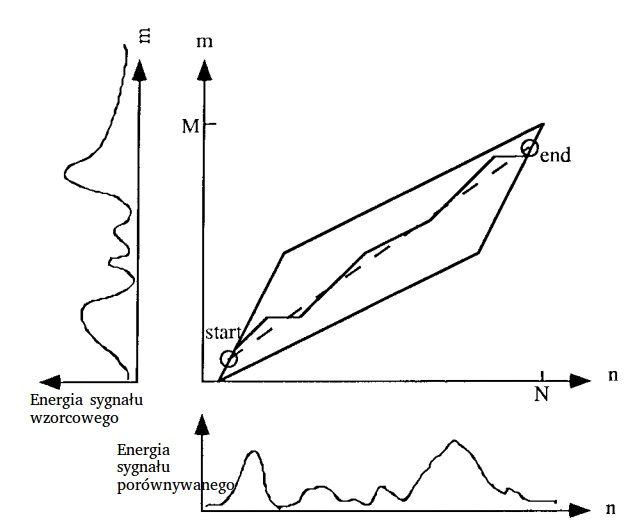
\includegraphics[width=0.6\textwidth]{dtwspeech.jpg}
    \caption{Rezultat działania metody DTW na bardziej skomplikowanej sekwencji.} Adaptacja z artykułu \cite{campbell}. Na głównym wykresie widać trajektorię z zaznaczonym ograniczeniem dla ścieżki algorytmu.
\end{figure}
Ze względu na wspomniane ograniczenia w zastosowaniu podana metoda nie jest już chętnie stosowana w systemach rozpoznawania mówcy. Dodatkową wadą jest duża złożoność obliczeniowa, szczególnie w przypadku dużej ilości sekwencji do sprawdzenia. Jego skuteczność maleje wraz ze wzrostem długości sekwencji. Zaletą tego rozwiązania jest jednak prostota implementacji i w zastosowaniach z detekcją krótkich haseł metoda może okazać się być skuteczna.

\subsection{Kwantyzacja wektorów - VQ.}
\label{vq}

Inną deterministyczną metodą (\textit{ang. template model}) stosowaną w etapie dopasowania wzorca w problemach rozpoznawania mówcy jest kwantyzacja wektorów (\textit{ang. vector quantization}). W odróżnieniu do wcześniej omawianej metody DTW, ta technika jest jest niezależna od kolejności analizowanych wektorów cech - tzn. jest niezmienny w czasie (\textit{ang. time-invariant)}. Z tego powodu możliwe jest zastosowanie tej techniki dla systemów rozpoznawania mówcy niezależnego od wypowiadanego tekstu (\textit{ang. text-independent}). 
Technika kwantyzacji wektorów należy do klasy problemów z zakresu technik dopasowania wzorca jaką jest uczenie bez nadzoru  (\textit{ang. unsupervised learning}). Tego typu problem nazywany jest także \cite{fosr} klasteryzacją (\textit{ang. clustering}). Jest to zagadnienie analizy skupień to znaczy dokonywane jest grupowanie przestrzeni elementów na którą składa się większa ilość - w przypadku rozpoznawania mówcy - wektorów cech na mniejszą ilość regionów. Regiony te reprezentowane są przez pewien ustalony wektor wzorcowy $ \tilde{x}$. Zatem każdy punkt rozpatrywanej przestrzeni wektorów cech - $x$, należy do regionu reprezentowanego przez wzorcowy wektor, względem którego ów punkt leży najbliżej w rozumieniu wybranej, zdefiniowanej na tej przestrzeni metryki $d(x,\tilde{x})$.
W fazie testowania, przeprowadzana jest analiza przynależności wektorów wejściowych do regionów reprezentujących weryfikowanego mówcę, to znaczy obliczana jest suma ich odległości do najbliższego wektora wzorcowego:
\begin{equation}
  z = \sum_{j=1}^{L} \min_{\tilde{x} \in  C} \left\{ d(x_j, \tilde{x}) \right\}. 
\end{equation}
Funkcja ta wyraża miarę dopasowania wektorów wejściowych do weryfikowanego modelu mówcy. 
W tej metodzie zbiór wektorów reprezentujących poszczególnych mówców nazywany jest książką kodową (\textit{ang. codebook}), zaś każdy wektor wchodzący w jej skład nazywa się kodem lub hasłem (\textit{ang. codeword}).

Przykładowy proces klasteryzacji w procesie uczenia się został przedstawiony na rysunku \ref{VQjpg}. Z puli 5000 wektorów akustycznych cech został stworzony model mówcy reprezentowany przez 64 wektory wzorcowe - tzw. \textit{codebook}.

\begin{figure}[ht!]
  \centering
    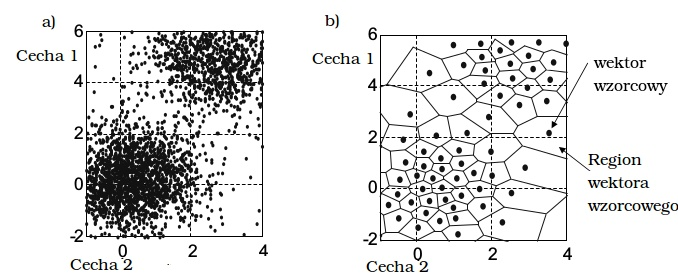
\includegraphics[width=0.8\textwidth]{overwiewVQ.jpg}
    \label{VQjpg}
    \caption{Klasteryzacja przestrzeni. Adaptacja z artykułu \cite{overview}. Na rysunku zostały przedstawione tylko 2 arbitralnie wybrane wymiary z wektora cech. Dane uczące składające się z 5000 wektorów zostały przekształcone na model 64 wektorów wzorcowych w procesie kwantyzacji wektorów.}
\end{figure}

Metoda ta cechuje się tym, że nie przechowuje informacji związanej z sekwencją wypowiedzi, więc nie jest w stanie wychwycić pewnych cech związanych z konkretnym przejściem pomiędzy kolejnymi segmentami mowy. Z drugiej strony upraszcza w sposób znaczący implementację systemu.


W tej pracy metoda kwantyzacji wektorów została użyta w przykładowej implementacji systemu weryfikacji mówcy w postaci realizującego nią algorytmu LGB.

\subsubsection{Algorytm LGB.}
\label{lgb}

\begin{figure}
  \centering
    \input{lbz.pgf}
    \caption{\label{lgbvis} Wizualizacja procesu podwajania i aktualizacji pozycji w algortymie LBZ.}
\end{figure}

Algorytm Linde, Buzo i Greya - LGB \cite{linde} przedstawia sposób uzyskania wektorów wzorcowych (ksiązki kodów - "codebook") reprezentujących mówcę, uzyskanego z danych uczących zawierających dużą ilość wektorów cech wyekstrahowanych z wypowiedzi modelowanego mówcy. Jest to algorytm szeroko znany i chętnie wykorzystywany \cite{minidsp} w zadanie rozpoznawania mówcy. Zaczynając od jednego punktu, np. uśrednionego wektora cech (jak we wzorze \ref{centroid}) produkowane są kolejne centroidy poprzez podział. Ten algorytm więc produkuje książkę kodów o rozmiarze K gdzie K jest potęgą dwójki. W kolejnych etapach algorytmu dokonuje się detekcji najbliższej centroidy dla każdego wektora cech danych trenujących. Ze względu na nowo powstałe regiony aktualizuje się położenie centroid. Po każdej aktualizacji jest prawdopodobne, że kolejne wektory cech zmienią swój region klasteryzacji, a zatem proces powtarza się aż do ustabilizowania się tychże regionów. Następnie powtarza się podwajanie wektorów wzorcowych aż do uzyskania pożądanej ich ilości K. Poniżej podsumowano w sposób szczegółowo kolejne etapy algorytmu, na rysunku \ref{lgbblock} przedstawiono schemat blokowy algorytmu, a na rysunkach \ref{lgbvis} przedstawiono wizualnie kolejne etapy przetwarzania algorytmu dla dwóch arbitralnie wybranych wymiarów z wektorów cech.
\\


\begin{figure}[ht!]
  \centering
    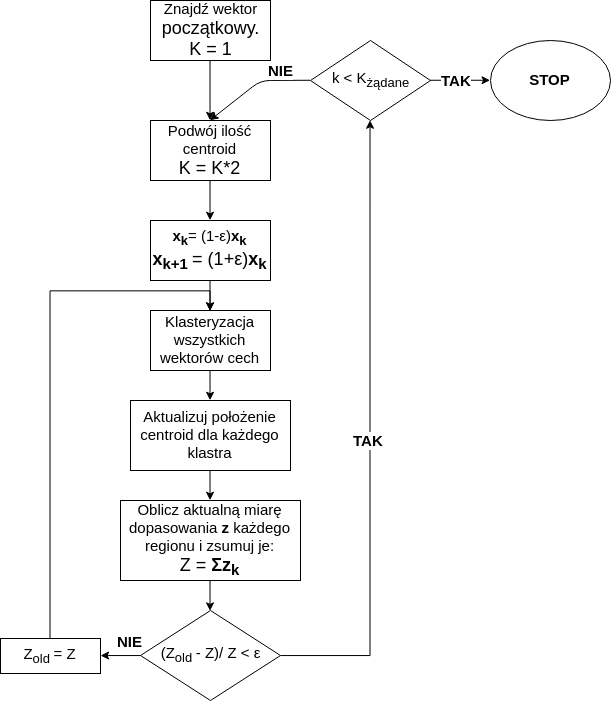
\includegraphics[width=1\textwidth]{lbgdiagram.png}
    \label{lgbblock}
    \caption{Schemat blokowy algorytmu Linde, Buzo i Greya. \cite{minidsp}}
\end{figure}

\textbf{Kolejne kroki algorytmu Linde, Buzo i Greya.\cite{minidsp}}
\begin{enumerate}
  \item Utwórz jedno-elementową książkę kodów - zawierającą uśrednioną centroidę jak we wzorze \textbf{\ref{centroid}} dla wszystkich treningowych wektorów cech.
  \item Podwój ilość elementów w książce kodów. Zmodyfikuj ich poszczególne wartości ze względu na wybrany, mały czynnik $\epsilon$ w następujący sposób, dla każdego \textbf{k} gdzie \textbf{$ k \in \{1,...,K\}$}:
    \begin{itemize}
      \item $ \bm{\tilde{x}_k} = (1 - \epsilon) \cdot \bm{\tilde{x}_k} $,
      \item $ \bm{\tilde{x}_{k+1}} = (1 + \epsilon) \cdot \bm{\tilde{x}_k} $.
    \end{itemize}
    Co oznacza przesunięcie je w przeciwnych kierunkach (w N-wymiarowej przestrzeni).
  \item Dokonaj klasyfikacji wszystkich wektorów trenujących - znajdź dla każdego najbliższą centroidę w rozumieniu przyjętej metryki $ d(\bm{\tilde{x}_k}, \bm{x})$. 
  \item Zaktualizuj położenie każdej centroidy jako średniej \textbf{\ref{centroid}} ze wszystkich wektorów cech sklasyfikowane jako leżące najbliżej.
  \item Powtarzaj kroki 3 i 4 dopóki położenie nowych centroid nie ustabilizuje się (różnica przesunięcia dwóch ostatnich iteracji jest poniżej ustalonego progu).
  \item Powtarzaj kroki 2, 3, 4 i 5 do momentu otrzymania słownika o żądanej długości \textbf{K}.
\end{enumerate}


\subsection{Mikstury Gaussowskie - GMM.}
Techinka modelowanie miksturami Gaussowskimi {\textit{ang. Gaussian mixture modeling}} jest metodą stochastyczną rozpoznawania wzorca. GMM jest sposobem modelowania uważanym za swego rodzaju standard w metodach rozpoznawania mówcy niezależnym od wypowiadanego tekstu. Tak jak wspomniano w rozważaniach ogólnych (\ref{featurematching}), w metodach probabilistycznych należy ustalić funkcję gęstości prawdopodobieństwa $p(X|\lambda)$ charakteryzującą danego mówcę. Dla problemu rozpoznawania mówcy niezależnego od tekstu, nie ma żadnej wiedzy apriori, którą można by było wykorzystać do założenia jakiegoś rozkładu. Dlatego też metoda GMM proponuje dokonania aproksymacji tzw. miksturami Gaussa (\textit{ang. Gaussian mixtures}). Okazuje się, że taka reprezentacja funkcji gęstości prawdopodobieństwa jest równie skuteczna co dużo bardziej skomplikowana reprezentacja ukrytymi modelami Markova (HMM) dla problemu rozpoznawania bez znajomości tekstu \cite{reynolds}, ze względu na brak przydatności wiedzy o sekwencji wektorów cech. Dla K-wymiarowych wektorów cech funkcja gęstości prawdopodobieństwa dla modeli GMM wyraża się jako:
\begin{equation}
  p(X|\lambda) = \sum^{M}_{i=1} w_ip_i(X).
\end{equation}
gdzie: $w_i$ są współczynnikami wagowymi ustalanymi w fazie uczenia oraz $\sum_{i=1}^{M} w_i =1$. M oznacza zaś liczbę wykorzystanych misktur Gaussowskich do aproksymacji funkcji gęstości prawdopodobieństwa dla modelu $ \lambda$. Kolejna mikstura Gaussowska przybiera postać wielowymiarowej funkcji rozkładu Gaussa:
\begin{equation}
  p_i(X)=\frac{1}{(2\pi)^{K/2} \cdot |\bm{\Sigma_i}|^{\frac{1}{2}}} \cdot \exp\left\{-\frac{1}{2}(X- \bm{\mu_i})'(\bm{\Sigma_i})^{-1}(X-\bm{\mu_i})\right\}
\end{equation}
gdzie: $\bm{\Sigma_i}$ oznacza macierz kowariancji wektora cech X, $\mu_i$ jest wektorem średnim (K-wymiarową wartością oczekiwaną). Pełny opis modelu $\lambda$ zapewnia zbiór parametrów $\lambda = \{w_i,\bm{\mu_i},\bm{\Sigma_i} \}$. Przy pomocy wektorów cech danych trenujących dokonywana jest estymacja parametrów dla poszczególnych mikstur Gaussowskich. W tym celu najczęściej używa się się metod maksymalnego prawdopodobieństwa a posteriori MAP (\textit{maximum a posteriori probability}) oraz algorytmu EM (\textit{ang. expectation-maximization}).
\subsection{Inne metody modelowania mówcy.}
\begin{itemize}
  \item{\textbf{Sztuczne sieci neuronowe} (\textit{ang. Artificial Neural Network - ANN})} - są metodą uczenia maszynowego wykorzystującą tzw. neurony będące strukturą matematyczną realizującą funkcję nieliniową o wielu wejściach i jednym wyjściu. Takie systemy mają zastosowanie w tworzeniu nowych metod zarówno w dziedzinie parametryzowania mowy (ekstrakcji cech) a także w dziedzinie modelowania mówcy. Tworzone są także systemy złożone z sieci neuronowych realizujące systemy rozpoznawania mówcy od początku do końca. Główną zaletą takich systemów z punktu widzenia wykonania zadania rozpoznawania w czasie rzeczywistym jest możliwość implementacji takiego algorytmu bezpośrednio na sprzęcie za pomocą układów FPGA.
  \item{\textbf{Maszyny wektorów wspierających} (\textit{ang. Support Vector Machine - SVM}) \label{svm}} - są metodą uczenia maszynowego służącą do rozwiązania zadania uczenia z nadzorowaniem. Stosowana jest z sukcesem dla cech niskiego i wysokiego poziomu. Szczególnie chętnie jest stosowany w zadaniu weryfikacji mówcy. Dla tego problemu metoda SVM w fazie trenowania korzysta z oznaczonych wektorów dla mówcy modelowanego w celu konstrukcji hiperpłaszczyzny rozdzielającej wektory należące do mówcy oraz wektory tła. Problem znalezienia takiej hiperpłaszczyzny jest problemem optymalizacji funkcji decyzyjnej postaci:
\begin{equation}
  f(\bm{X}) =\sum^N_{i=1}\alpha_it_iK(\bm{X},\bm{X_i}) + d
\end{equation}
    gdzie $\bm{x_i}$ - wektory wspierające, $t_i \in \{-1,1\}$ - oznaczenie przynależności wektorów, $\alpha$ waga wektora oraz funkcja jądra $K(\bm{X},\bm{X_i})$ określająca odległość od hiperpłaszczyzny $g(X)$.
    W najprostszym przypadku, klasyfikatora maksymalnego marginesu - (który był zaproponowany w oryginalnej pracy Vapnika \cite{vapniksvm}) maksymalizuje się odległość (margines) najbliższych wektorów $\bm{x_i}$ (czyli \textit{wektorów wspierających}  (\textit{ang. support vectors})) do wspomnianej hiperpłaszczyzny  $g(X)$. W wyniku uzyskiwany jest model - granica oddzielająca mówcę od tła.
  \item{\textbf{Fuzja} (\textit{ang. fusion})} - dla problemu rozpoznawania mówcy zostały zastosowane systemy korzystające z kombinacji różnych typów wektorów cech sparametryzowanego sygnały mowy. Realizowane są również systemy korzystające z różnych modeli uzyskanych na podstawie tych samych wektorów cech. Decyzja na wyjściu takiego systemu jest podejmowana za pomocą funkcji uwzględniające wyniki wszystkich zastosowanych wewnętrznych systemów. Najlepsze rezultaty otrzymywane są gdy korzysta się z jak najbardziej niezależnych od siebie metod - tzn. uwydatniających różne właściwości sygnały mowy. Widoczne jest to szczególnie przy fuzji cech wysokiego i niskiego poziomu.
\end{itemize}
\section{Teoria decyzji}
\label{verif}

System weryfikacji mówcy uzupełnia zadanie rozpoznawania mówcy o etap weryfikacji - tzn. podjęcia decyzji o autoryzacji osoby podającej się za mówcę znajdującego się w bazie modeli systemu. Każdy system może popełnić dwa rodzaje błędów:
\begin{itemize}
  \item{\textbf{Błąd I rodzaju}} - pozytywna weryfikacja fałszywego mówcy,
  \item{\textbf{Błąd II rodzaju}} - negatywna weryfikacja prawdziwego mówcy.
\end{itemize}
Intuicyjnie można powiedzieć, że błąd rodzaju I jest znacznie poważniejszy od błędu II rodzaju. Relacja częstotliwości tych błędów regulowana jest w większości metod za pomocą progu $\theta$. Pożądane jest zatem zwykle przyjmowanie wartości progu w taki sposób aby minimalizować ten poważniejszy. Ze względów na wygodę i efektywność wymaga się także odpowiednio małego progu odrzuceń systemu. Z drugiej strony, tak jak opisano wcześniej w tej pracy (\cite{err}), poziom tych błędów może być miarą jakości działania systemu weryfikacji. Główną metodą w omawianych systemach jest testowanie hipotez w ujęciu bayesowskim, co jest przedstawione dalej.  

\subsection{Testowanie hipotez w zadaniu weryfikacji mówcy.}

Dla testowanego segmentu mowy $Y$ w zadaniu weryfikacji mówcy usiłuje się ustalić czy został on wyprodukowany przez mówcę $S$. Na potrzeby tego zadania można postawić dwie przeciwne wobec siebie hipotezy:
\begin{enumerate}
  \item{$\quad\bm{H_0}$}: sygnał mowy $Y$ pochodzi od mówcy $S$,
  \item{$\quad\bm{H_1}$}: sygnał mowy $Y$ nie pochodzi od mówcy $S$.
\end{enumerate}
Powszechnie w dziedzinie weryfikacji mówcy stosowane jest kryterium stosunku modeli prawdopodobieństwa $\lambda_S$ (\textit{ang. likelihood ratio}) sformułowane następująco:
\begin{equation}
  \label{likratio}
  \lambda_S = \frac{p(Y|H_0)}{p(Y|H_1)}
  \begin{cases}
    \ge \theta, \textrm{ przyjmij hipotezę } H_0 \\
    < \theta, \textrm{ odrzuć hipotezę } H_0
  \end{cases}
\end{equation}
gdzie funkcje $p(Y|H_0)$ i $p(Y|H_1)$ oznaczają warunkowe funkcje gęstości prawdopodobieństwa dla sygnału Y, $\theta$ oznacza prób przyjęcia. 

Mając jednak na uwadze klasycznie podejście od problemu - zawierające etapy ekstrakcji cech/parametryzacji sygnału mowy \textbf{\ref{featureextraction}} oraz modelowania mówcy \textbf{\ref{featurematching}} - oczekujemy, że z sygnału $Y$ zostanie wyekstrahowany zbiór cech $X = \{x_1,...,x_T\}$ dla kolejnych chwil czasu $t = \{1,...,T\}$. Z tego powodu \textbf{\ref{likratio}} można zapisać jako:

\begin{equation}
  \lambda_S = \frac{p(X|\lambda_S)}{p(X|\lambda_{\tilde{S}})}
  \begin{cases}
    \ge \theta, \textrm{ przyjmij hipotezę } H_0 \\
    < \theta, \textrm{ odrzuć hipotezę } H_0
  \end{cases}
\end{equation}
taka postać współczynnika uwarunkowana jest tym, że funkcja gęstości prawdopodobieństwa jest scharakteryzowana przez zbiór cech $X$ sparametryzowanej mowy $Y$, a hipoteza $\bm{H_0}$ jest reprezentowana przez model mówcy $S$ - $\lambda_{S}$  oraz hipoteza $\bm{H_1}$ jest zdefiniowana przez model odniesienia $\lambda_{\tilde{S}}$.

W ostateczności jako kryterium decyzji używa się logarytmu wspomnianego czynnika $\log \left( \lambda_S \right)$ (\textit{ang. log likeligood ratio}). Ostatecznie omawiane kryterium przyjmuje postać:
\begin{equation}
  \label{loglike}
  \Lambda(X)= \log({p(X|\lambda_S)}) - \log({p(X|\lambda_{\tilde{S}})}
  \begin{cases}
    \ge \theta, \textrm{ przyjmij hipotezę } H_0 \\
    < \theta, \textrm{ odrzuć hipotezę } H_0
  \end{cases}
\end{equation}

Model odniesienia $\lambda_{\tilde{S}}$ zazwyczaj przybiera jedną z dwóch form:
\begin{itemize}
  \item{Model tła (\textit{ang. background model})} - używa się przekształcenia $\mathcal{F}(p_1(X|\lambda_1),...,p_N(X|\lambda_N))$ do skonstruowania jednego modelu tła i co za tym idzie funkcji gęstości prawdopodobieństwa $p(X|\lambda_{\tilde{S}})$. Jednym z najbardziej popularnych modeli tego typu jest UBM (\textit{ang. Universal Background Model}). Niewątpliwą korzyścią płynąca z zastosowania tej metody jest tylko jednokrotna operacja obliczenia modelu który stosowany jest dla wszystkich testów.
  \item{Model kohorty (\textit{ang. cohort})} - model odniesienia konstruowany jest za pomocą tylko najbliższych znanych modeli. Możliwy jest wybór $p(X|\lambda_{\tilde{S}})$ np. jako tego cechującego się największym prawdopodobieństwem dla realizacji X lub jako średni model towarzyszących modeli.
\end{itemize}

Podana metoda wykorzystywana jest z łatwością dla technik GMM i HMM modelowania. Jednak metody deterministyczne, w szczególności technika kwantyzacji wektorów (VQ) wymaga zastosowania dodatkowych, bardziej skomplikowanych technik z zakresu teorii decyzji aby wykorzystać opisywaną metodę. 

\subsection{Weryfikacja dla metod deterministycznych.}
\subsubsection{Stały próg.}
\label{fixed}
System weryfikacji mówcy korzystający z podstawowej wersji techniki kwantyzacji wektorów (VQ), z racji tego, iż nie jest modelem probabilistycznym oraz ze względu na prostotę, korzysta zwykle ze stałego progu $\theta$. Metoda jest odpowiednikiem weryfikacji mówcy z jednym mówcą tła. Przyjęty próg nie posiada jednak wymiaru prawdopodobieństwa. W przypadku VQ próg $\theta$ przyjmuje wartość związaną z przyjętą miarą dopasowania $D_{avg}(X, X_{\lambda})$. Przykładem takiego systemu jest system weryfikacji mówcy z wyświetlanym hasłem, opisany w \cite{10digits92}, na którym to wzoruje się prezentowany w niniejszej pracy przykład systemu. Próg dla takiego przypadku często wyznacza się empirycznie. 

\subsubsection{Próg dla modelu kohorty.}
Dla metod deterministycznych możliwe jest także wykorzystanie analogicznego warunku jak w \ref{loglike}, z tym, że zastępując warunkową funkcję gęstości prawdopodobieństwa przez funkcję miary dopasowania $D_{avg}(X_{\lambda}, X_{\tilde{\lambda}_{kohorta}})$, gdzie $X_{\tilde{\lambda}_{kohorta}}$ oznacza model uzyskany ze względu na mówców zawartych w kohorcie. Zatem podobnie jak poprzednio otrzymuje się:

\begin{equation}
  \label{loglikedis}
  d(X)= \log({D_{avg} (X, X_{\lambda}})) - \log(D(X, X_{\lambda_{kohorta}}))
  \begin{cases}
    \ge \theta, \textrm{ przyjmij hipotezę } H_0 \\
    < \theta, \textrm{ odrzuć hipotezę } H_0
  \end{cases}
\end{equation}

Dla metody SVM (\ref{svm}) zaś kryterium to może przyjąć postać:

\begin{equation}
  \label{loglikesvm}
  f(X)= \sum_{i\in\{i|t_i = 1\}} \alpha_i K(\bm{X},\bm{X_i}) - \sum_{i\in\{i|t_i = 1\}}\alpha_i K(\bm{X},\bm{X_i)} + d
  \begin{cases}
    \ge \theta, \textrm{ przyjmij hipotezę } H_0 \\
    < \theta, \textrm{ odrzuć hipotezę } H_0
  \end{cases}
\end{equation}

\subsection{Przycinanie mówców\\ (\textit{ang. speaker pruning}).}

\textit{Speaker pruning} (tzn. 'przycinanie mówców') jest techniką wspomagającą zadanie identyfikacji mówcy w zastosowaniach czasu rzeczywistego. Możliwe jest też zastosowanie tej metody dla problemu weryfikacji mówcy korzystającego z modelu kohorty, który wymaga analizy więcej niż jednego modelu odniesienia w czasie rzeczywistym czyli tzw. (\textit{ang. unconstrained cohort normalization}). Omawiana technika ta polega na odrzucaniu nieprawdopodobnych mówców już w trakcie nadchodzenia kolejnych wektorów cech, sparametryzowanego sygnału mowy. Najczęściej przyjmuje się pewien krok ilości nowych wektorów które będą wykorzystane do wstępnego odrzucenia kolejnych nieprawdopodobnych modeli. Przykładem algorytmu dla zastosowaniu w \ref{loglikedis} jest algorytm szybkiego dobierania kohorty (\textit{ang. Fast Cohort Scoring - FCS}) \cite{finprunning}. Algorytm korzysta z wcześniej opisanego algorytmu LGB \ref{lgb}, klasteryzując zbiór wektorów $X$ na mniejszy $\tilde{X} = LBG(X)$. Niech $\lambda$ oznacza zbiór centroid modelu. Dokonywany jest wybór $K$ najbliższych mówców ze względu na miarę podobieństwa $D_{avg}(\tilde{X},\lambda)$. Zbiór wybranych modeli jest wspomnianą kohortą. W ostatnim kroku tego algorytmu oblicza się wartość kryterium d(X) z \ref{loglikedis} jako:
\begin{equation}
  d(X) = \frac{D_{avg}(\tilde{X},\lambda)}{\frac{1}{K}\sum_{k=1}^{K}D_{avg}(\tilde{\tilde{X}},\lambda_k)}
\end{equation}

\chapter{Projekt architektury oprogramowania}

W tym rozdziale przedstawiono architekturę oprogramowania systemu weryfikacji mówcy w czasie rzeczywistym w przeznaczeniu dla systemów wbudowanych. W pierwszej kolejności zaprezentowano ogólną struktura zadania weryfikacji mówcy odpowiednio dla fazy modelowania oraz fazy testowania, na której to opiera się cały projekt. Następnie przedstawiono szczegółowy opis zaproponowanej architektury dla aplikacji algorytmów weryfikacji mówcy w czasie rzeczywistym. Dodatkowo
zaprezentowano ogólną implementację rozwiązania problemu dla języka C++ - omówiono struktury i algorytmy sterujące znajdujące się w systemie, które są niezależne od wybranych metod z zakresu weryfikacji mówcy. Przykład konkretnego zastosowania omawianej architektury oraz opis implementacji w pełni funkcjonalnego sytemu weryfikacji mówcy znajduje się w kolejnym rozdziale.


\section{Schemat funkcjonalny systemu weryfikacji mówcy}
\label{funcioniert}

W ogólności system weryfikacji mówcy musi sprostać dwóm problemom składającym się na dwa etapy niezależne w czasie: uzyskania modelu mówcy w fazie modelowania (treningu) oraz podjęcie decyzji o weryfikacji mówcy na podstawie wcześniej uzyskanego modelu oraz testowanego sygnału mowy w fazie testowania (weryfikacji). Ponieważ te dwa etapy różnią się na poziomie funkcjonalności zatem struktura wewnętrzna systemów również w pewnym stopniu są różne.

\subsection{Faza modelowania}

Aby system mógł podjąć decyzję o weryfikacji mówcy w jego posiadaniu musi znajdować się wcześniej uzyskany model weryfikowanego mówcy, który wykorzystywany jest do porównania z odpowiednio sparametryzowanym, testowym sygnałem mowy. Odbywa się to w etapie modelowania. Ogólna struktura procesu uzyskiwania modelu mówcy z uwzględnieniem przepływu danych znajduje się na rysunku {\ref{fig:fundiagmodel}}. Zadanie uzyskania modelu mówcy składa się kolejno z etapów:

\begin{figure}[ht!]
  \centering
    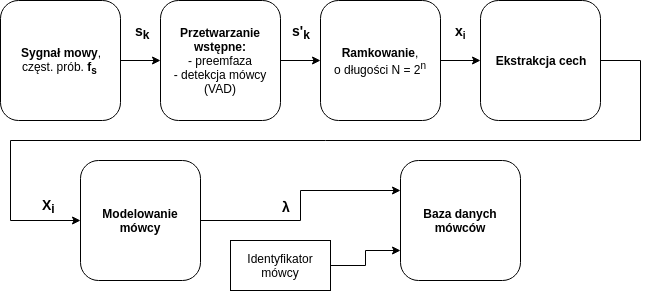
\includegraphics[width=0.9\textwidth]{./fundiagmodel.png}
    \caption{\label{fig:fundiagmodel} Schemat funkcjonalny systemu weryfikacji mówcy dla etapu modelowania.}
\end{figure}

\begin{enumerate}
\item{\textbf{Akwizycja sygnału mowy}} - wejściem całego sygnału jest spróbkowany z częstotliowścią $f_s$ sygnał mowy $\bm{s_k}$. Dostarczany jest on bądź to z pamięci komputera jako całość lub dostarczany jest w czasie rzeczywistym jako kolejne próbki. Dla tego drugiego przypadku na ten etap składa się realizacja sprzętowa akwizycji sygnału akustycznego mowy za pomocą przetwornika elektroakustycznego oraz przetwornika analogowo-akustycznego. Ważnym elementem jest również odpowiednie filtrowanie
    analogowe sygnału - usunięcie składowej stałej oraz filtrowanie częstotliwości wyższych od połowy częstotliwości próbkowania $f_s$ (filtracja antyaliasingowa).
\item{\textbf{Przetwarzanie wstępne}} - na ten etap mogą składać się wszelkiego rodzaju techniki poprawy jakości sygnału takie jak odszumianie. Najczęściej w systemach weryfikacji mówcy stosuje się tzw. preemfazę - czyli wzmacnianie wyższych częstotliwości sygnału oraz systemy detekcji mówcy (\textit{ang. Voice Activity Detection - VAD})  zwłaszcza dla systemów czasu rzeczywistego. W wyniku przeprowadzonych operacji z sygnału $\bm{s_k}$ otrzymujemy przetworzony sygnał $\bm{s'_k}$.
\item{\textbf{Ramkowanie}} - zwykle w przypadku ekstrakcji cech niskiego poziomu konieczne jest zaaplikowanie ramek na sygnał mowy tak, aby uzyskać chwilowe wektory cech. Dla metod ekstrakcji cech wykorzystujących dyskretne przekształcenie Fouriera (DFT) zwykle dobiera się ramki o długościach równymi $N=2^n$, gdzie n - liczba całkowita. W przypadku takich cech jak LPCC nie jest to warunek konieczny, jednak często stosowany. W wyniku operacji ramkowania otrzymywany jest zbiór wektorów $\bm{x_i}$ o długości N.
\item{\textbf{Ekstrakcja cech}} - na ten etap składa się przetwarzanie ramek sygnału mowy $\bm{x_i}$ na wektory cech oznaczone jako $\bm{X_i}$. Różne techniki wykorzystywane w tym procesie opisano w rozdziale {\ref{featureextraction}}.
\item{\textbf{Modelowanie mówcy}} - w tej części konstruowany jest model mówcy $\bm{\lambda}$ na podstawie zbioru wektorów trenujących $\bm{X_i}$. Różne techniki otrzymywania modeli opisane zostały w rozdziale {\ref{featurematching}}. Model reprezentowany jest najczęściej jako wektor współczynników: w VQ są to centroidy znajdujące się w przestrzeni wektorów, zaś w technice GMM są tą współczynniki wagowe $w_i$ kolejnych funkcji aproksymujących funkcję gęstości prawdopodobieństwa.
\item{\textbf{Zapisanie modelu do bazy danych}} - Wartości parametrów charakteryzujących model mówcy $\bm{\lambda}$ muszą być zapisane na potrzeby fazy weryfikacji. Konieczne jest, aby wraz z modelem została zapisana informacja dotycząca tożsamości mówcy - może być to numer identyfikacyjny w postaci danych charakterystycznych dla mówcy. Identyfikator mówcy jest wykorzystywany w fazie weryfikacji razem z modelem.
\end{enumerate}

\label{pies}

\subsection{Faza weryfikacji.}

Jeżeli system jest w posiadaniu modelu mówcy, za który podaje się mówca, od którego testowany sygnał mowy pochodzi, system weryfikacji mówcy może przeprowadzić procedurę weryfikacji. W tym celu musi przedstawić informację identyfikującą weryfikowanego mówcę. Ogólna struktura procesu weryfikacji mówcy z uwzględnieniem przepływu danych znajduje się na rysunku {\ref{fig:fundiagverif}}. W omawianej procedurze zachowana jest postać algorytmu (rozdział \ref{pies}) aż do momentu uzyskania zbioru wyekstrahowanych cech włącznie. Natomiast zachodzą istotne zmiany co do kolejnych etapów:

\begin{figure}[ht!]
  \centering
    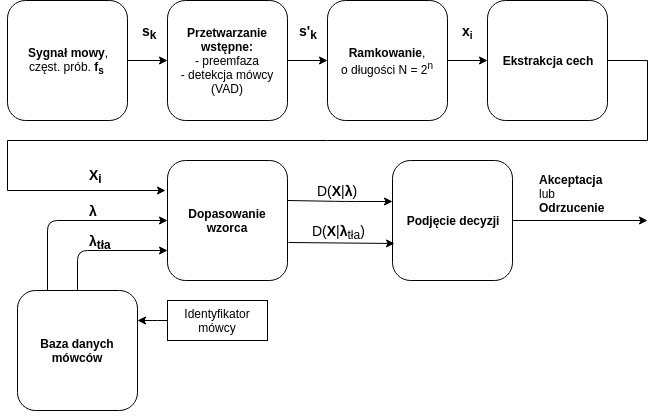
\includegraphics[width=1\textwidth]{./fundiagverif.png}
    \caption{\label{fig:fundiagverif} Schemat funkcjonalny systemu weryfikacji mówcy dla fazy weryfikacji.}
\end{figure}

\begin{enumerate}
    \item{\textbf{Dopasowanie wzorca}} - ten etap korzysta ze zbioru cech $X_i$ w celu weryfikacji mówcy. Podczas tego etapu obliczana jest miara dopasowania pomiędzy wektorami $X_i$ a modelami kolejno $\lambda$ i $\lambda_{tla}$. W tym przypadku model oznaczony jako $\lambda_{tla}$ oznacza albo model tła albo model kohorty (w rozumieniu rozdziału {\ref{verif}}). Wyjściem procesu jest wartość liczbowa tej miary dla obu porównań na rysunku oznaczone jako $D(\bm{X}|\bm{\lambda})$ i $D(\bm{X}|\bm{\lambda}_{tla})$. Dla techniki VQ miara dopasowania to wartość funkcji metryki $d(X,C_n)$ gdzie $C-n$ to centroidy modelu. W przypadku techniki GMM miarą dopasowania jest prawdopodobieństwo.
\item{\textbf{Podjęcie decyzji}} - ostatnim etapem razy weryfikacji mówcy jest podjęcie decyzji. Techniki związane z tym zagadnieniem opisano w rozdziale {\ref{verif}}. Decyzja podejmowana jest na podstawie dwóch liczb dostarczonych z poprzedniego bloku: $D(\bm{X}|\bm{\lambda})$ i $D(\bm{X}|\bm{\lambda}_{tla})$ oraz ustalonego przez projektanta progu $\theta$. Wyjściem całego systemu jest zmienna binarna przyjmująca wartości: Akceptacja lub Odrzucenie.
\end{enumerate}

\section{Architektura systemu weryfikacji mówcy dla czasu rzeczywistego}

Na podstawie przedstawionych schematów funkcjonalnych została zaproponowana architektura oprogramowania dla przetwarzania w czasie rzeczywistym. Ogólny schemat został przedstawiony na rysunku {\ref{fig:overallrt}}. Rozwiązanie oparte jest na użyciu trzech bloków przetwarzania oraz trzech buforów typu fifo (\textit{ang. first in firts out}). Projekt oparty jest na podejściu producent-konsument, tzn. występuje blok produkujący dane przekazywane do kolejki FIFO - nazwany producentem oraz blok
odbierający dane z kolejki FIFO - nazwany konsumentem.  W omawianym rozwiązaniu zawsze występuje tylko jeden producent i jeden konsument. Takie bloki mogą zostać zaimplementowane w zwykłym systemie operacyjnym jako wątki, w systemie czasu rzeczywistego jako 'taski' oraz sekwencyjnie w przypadku braku takiego wsparcia ze strony systemu uruchomieniowego. 

\begin{figure}[ht!]
  \centering
    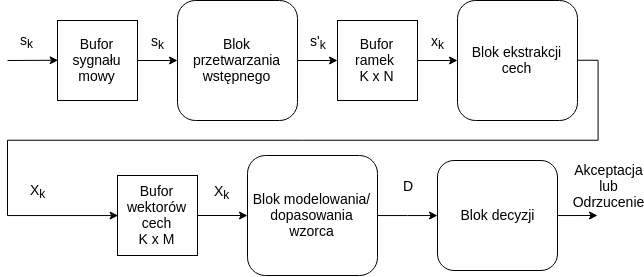
\includegraphics[width=1\textwidth]{./overallrt.png}
    \caption{\label{fig:overallrt} Schemat funkcjonalny architektury systemu weryfikacji dla przetwarzania w czasie rzeczywistym.}
\end{figure}

\subsection{Bufory FIFO}

Głównym zadaniem użytego w systemie buforu typu FIFO (kolejki) jest kontrola przepływu danych. Stan przepełnienia lub wyczerpania kolejki stanowi podstawę do sterowania kontekstem wykonywanego zadania. W systemie występują trzy kolejki przystosowane do różnego typu danych:
\begin{itemize}
\item{\textbf{Bufor sygnału mowy}} - jest to bufor FIFO przechowujący kolejne, nadchodzące próbki sygnału mowy. Może być zrealizowany programowo - dodatkowy wątek lub blok programu odpowiedzialny jest za jej napełnianie poprzez wywołanie odpowiednich wywołań systemowych lub za pomocą przerwania. Blok przetwarzania wstępnego jest w tym przypadku konsumentem i odbiera kolejne próbki z kolejki.
\item{\textbf{Bufor ramek}} - jest to bufor FIFO przechowujący kolejne ramki sygnału o stałym rozmiarze $N$. Ramki produkowane są przez blok przetwarzania wstępnego i wysyłane do tejże struktury danych. Odbiorcą jest blok ekstrakcji cech.
\item{\textbf{Bufor wektorów cech}} - jest podobny do buforu ramek, różni się jedynie mniejszym rozmiarem ramki dla wektora cech o długości $M$. 
\end{itemize}

\subsubsection{Implementacja kolejki FIFO}

Kolejki różnią się implementacją w zależności od wybranego systemu uruchomieniowego:
\begin{itemize}
\item{\textbf{System czasu rzeczywistego - RTOS}} - w tego typu systemach znajdują się gotowe implementacje kolejek przystosowane do synchronizacji pomiędzy taskami. Przykładem takiej struktury jest \textit{xQueue} w systemie operacyjnym \textit{FreeRTOS} \cite{freertos}.
\item{\textbf{Wielowątkowy system operacyjny}} - ponieważ w bibliotece standardowej nie znajdują się struktury danych umożliwiające bezpieczną pracę w środowisku wielowątkowym potrzebna jest inna implementacja kolejki niż standardowa \textit{stdqueue}. Implementacja może pochodzić z zewnętrznej biblioteki takiej jak \textit{boost} albo \textit{QT}. Jednak łatwo jest zaimplementować omawianą strukturę danych przy pomocy algorytmu wzajemnego wykluczenia (\textit{ang. mutex}) znajdującego się w
    bibliotece standardowej pod nazwą - \textit{std::mutex}. Poniżej podano przykładową implementację, z której korzysta się w przykładowym systemie opisanym w niniejszej pracy.
\begin{lstlisting}[style=lst:cpp, caption=Bezpieczna wątkowo kolejka\label{lst:queue}]
template <class T>
class queue
{
  public:
  ...
    T pop()
    {
      //zajecie mutexu
      std::unique_lock<std::mutex> mutex_lock(mutex_);
      while(queue_.empty()) // zablokuj watek jesli pusta
      {
        condition_.wait(mutex_lock);
      }
      auto item = queue_.front(); // pobierz element
      queue_.pop(); //usun obiekt z kolejki
      return item;
    }

    void push(T&& object)
    {
      //zajecie mutexu
      std::unique_lock<std::mutex> mutex_lock(mutex_);
      queue_.push(std::move(item)); // dodaj obiekt na koniec kolejki
      mutex_lock.unlock(); // zwolnij mutex
      condition_.notify_one(); // zaktualizuj zmienna condition_
    }
  ...

  private:
    std::queue<T> queue_;
    mutable std::mutex mutex_;
    std::condition_variable condition_;
};
\end{lstlisting}

Dla podanej implementacji zachowano podobną semantykę wezwań, tak jak w przypadku kolejki \textit{std::queue}: funkcja \textit{pop()} zwraca pierwszy element kolejki, zaś funkcja \textit{push()} umieszcza obiekt na końcu kolejki. Aby zapobiec zjawisku wyścigu użyta została blokada \textit{std::mutex} podczas odczytu i zapisu z kolejki. Z kolei obiekt \textit{std::condition\_variable} z biblioteki standardowej realizuje blokadę wątku odczytującego w przypadku, kiedy kolejka jest pusta. Wywołanie
        w linii 25 informuje zablokowany wątek o uzupełnieniu kolejki o jeden element. Pętla w linii 10 zapobiega zwolnieniu wątku w przypadku, gdy wystąpi inny powód odblokowania wątku niż powiększenie się kolejki.


\item{\textbf{Brak systemu uruchomieniowego}} - w przypadku braku środowiska wielowątkowego nie jest potrzebne zapewnienie kontenera bezpiecznego wątkowo (\textit{ang. thread safe}). Dlatego wystarczy wykorzystać gotową strukturę kolejki z biblioteki standardowej \textit{std::queue}.
\end{itemize}

\subsubsection{Kolejność wykonywania bloków}

W przypadku korzystania ze wsparcia systemu operacyjnego sprawa jest najprostsza - kolejne bloki implementowane są jako niezależne wątki synchronizowane za pomocą kolejek. Jeżeli jednak system nie korzysta ze wsparcia środowiska uruchomieniowego potrzebna jest implementacja odpowiedniej logiki sterującej. Na rysunku {\ref{fig:logics}} przedstawiono propozycję algorytmu sterowania wykonaniem w tego typu systemie.

\begin{figure}[ht!]
  \centering
    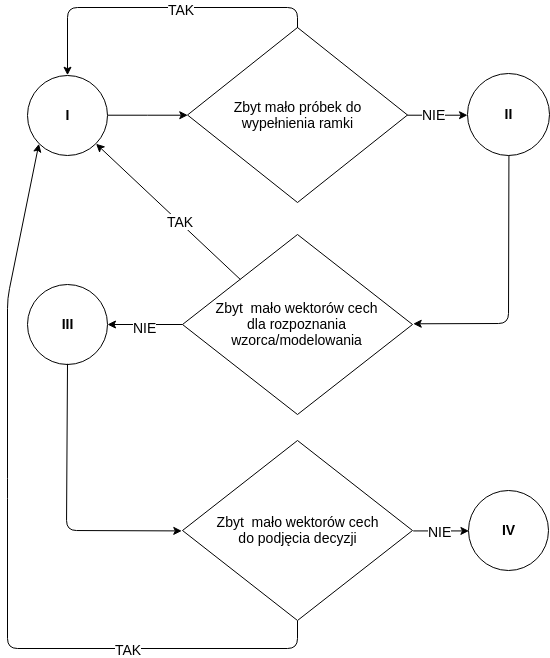
\includegraphics[width=0.6\textwidth]{./logic.png}
    \caption{\label{fig:logics} Algorytm sterownia bez wsparcia systemu operacyjnego. \textbf{Blok I} - blok wstępnego przetwarzania. \textbf{Blok II} - blok ekstrakcji cech. \textbf{Blok III} - blok rozpoznania wzorca/modelowania. \textbf{Blok IV} - blok podejmowania decyzji.}
\end{figure}

\subsection{Bloki przetwarzania}
Poniżej opisano trzy bloki przetwarzania znajdujące się w systemie. Bloki realizują funkcjonalności, które opisano w {\ref{funcioniert}}.
\begin{itemize}
\item{\textbf{Blok wstępnego przetwarzania}} - realizuje funkcjonalności przetwarzania wstępnego oraz ramkowania z rysunku {\ref{fig:fundiagverif}}. Wszystkie wykorzystywane funkcje w tym bloku zdefiniowane są w przestrzeni nazw \textit{dsp\_utils}. 
\item{\textbf{Blok ekstrakcji cech\label{archfeatureextraction}}} - realizuje funkcjonalność ekstrakcji cech. 
\item{\textbf{Blok rozpoznawania wzorca/modelowania\label{archpatternmatching}}} - realizuje funkcjonalność dopasowania wzorca oraz modelowania.
\item{\textbf{Blok podejmownia decyzji}} - realizuje funkcjonalność podejmowania decyzji o weryfikacji.
\end{itemize}


\subsection{Baza danych mówców}
Dany mówca reprezentowana jest jako następująca struktura danych dla systemu weryfikacji mówcy z wyświetlanym hasłem:
\begin{lstlisting}[style=lst:cpp, caption=struktura danych przechowująca informację o mówcy\label{lst:database}]
template <int C, int K>
using codebook_array = typename std::array<std::array<double, K>, C>; 


class speaker {
  public:
    speaker(const std::string& name)
      : speaker_info{name} {}  

    std::string name() {return speaker_info.name;};

    struct Code{
      Code(const std::string& text, codebook_array<C,K>&& code)
        : centroids{code}, text{text} {}
      std::array<std::array<double, K>, C> centroids;
      std::string text;
    };

    void add_code(speaker::Code&& code)
    {
      codebook.push_back(code); 
    }

  private:
    std::vector<Code> codebook;

    struct speaker_info{
      speaker_info(const std::string& name)
        : name{name} {}
      std::string name;
    } speaker_info;
};
\end{lstlisting}

Klasa \textit{speaker} zawiera dwie struktury danych: instancję struktury \textit{speaker\_info}, która reprezentuje numer identyfikacyjny mówcy przy pomocy zmiennej łańcuchowej \textit{name} oraz instancji struktury \textit{codebook} przechowującej wektory współczynników charakteryzujących modele (w przypadku metody VQ są to centroidy - stąd nazwa zmiennej \textit{centroids}). Alias do tablicy dwuwymiarowej, z której korzysta implementacja to \textit{codebook\_array}.

\chapter{System weryfikacji mówcy}

W tym rozdziale zostanie opisana implementacja pełnego systemu weryfikacji mówcy. 

\section{Platforma uruchomieniowa}

Weryfikacja poprawności działania systemu i wstępna implementacja zostały wykonane przy pomocy środowiska obliczeniowego Matlab. Rozwijanie oprogramowania w języku C++ na bazie narzędzi GNU odbywało się na systemie operacyjnym linux w dystrybucji debianowej. Docelową platformą uruchomieniową był komputer jednopłytkowy również z systemem takiego typu.

\section{Wybór technologii}

Omawiany system wykonuje parametryzacji sygnału mowy przy pomocy techniki Cepstralnych Współczynników Melowych (MFCC) w sekcji \textbf{\ref{mfcc}}. Rozpoznanie wzorca jest realizowane przy pomocy techniki kwantyzacji wektorów (VQ) (\textbf{sekcja \ref{vq}}), zaś proces modelowania mówcy dodatkowo korzysta z algorytmu LGB (\textbf{sekcja \ref{lgb}}).

\subsection{Sposób implementacji algorytmów}

Do implementacji algorytmów skorzystano ze znajdującej się w standardzie C++ bibliotek STL (Standard Template Library). W omawianej implementacji wykorzystywane są głównie trzy funkcje pochodzące z biblioteki STL są to:
\begin{itemize}
  \item{\textbf{std::generate(container\_iter start, container\_iter end, object\_func lambda)}} - funkcja generuje wartość dla każdego elementu pomiędzy iteratorem \textit{start} a iteratorem \textit{end} w jednym kontenerze za pomocą obiektu funkcyjnego \textit{lambda}.
  \item{\textbf{std::transform(container1\_iter start1, container1\_iter end1,
                       container2\_iter start2,
                       container3\_iter start3, object\_func lambda)}} 
  - funkcja generuje wartości w kontenerze o początku w \textit{start3} za pomocą obiektu funkcyjnego \textit{lambda} przyjmującego za argumenty kolejno wartości od start1 oraz od start2 aż do iteratora end1 i odpowiedniego w kontenerze nr. 2.
  \item{\textbf{std::for\_each(container\_iter start, container\_iter end, object\_func lambda)}} - produkuje wartości w kontenerze pomiędzy iteratorami start i end za pomocą obiektu funkcyjnego \textit{lambda} przyjmującego za argument wartości z tego kontenera. Funkcja może być zastąpiona pętlą zakresową: \textbf{for(auto \&\&x: container)}.

\end{itemize}

\section{Implementacja algorytmów wstępnego przetwarzania  sygnału mowy}

W tym miejscu została opisana implementacja bloku wstępnego przetwarzania opisanego w \textbf{sekcji \ref{archfeatureextraction}}.

\section{Implementacja ekstrakcji cech MFCC}

W tym miejscu została opisana implementacja bloku ekstrakcji cech opisanego w \textbf{sekcji \ref{archfeatureextraction}}.

Aby utrzymać wektory sparametryzowanego sygnały mowy w postaci współczynników MFCC nazleży wywołać funkcję \textit{mfcc\_extraction} przyjmującą za argumenty częstotliwość próbkowania \textit{samplerate} oraz wektor ramek o długości N z próbkami sygnału mowy \textit{speech\_frames}. Funkcja zwraca wektor tablic długości K cech MFCC:

\begin{lstlisting}[style=lst:cpp, caption=Implementacja funkcji mfcc\_extraction\label{lst:mfcc}]

  std::vector<std::array<double, K>>
  mfcc_extraction( std::vector<std::array<double, N>>&& speech_frames,
                   int samplerate)
  {
    (...)
\end{lstlisting}

    \subsubsection{Obliczanie widma mocy dla ramek oraz nałożenie filtrów mela}

Tak jak opisano w sekcji(\textbf{\ref{mfcc}}) pierwszym etapem ekstrakcji cech w tym przypadku jest obliczenie widma gęstości mocy. Kolejno w pętli wykonuje się operacje nakładania widma (za pomocą obiektu funkcyjnego \textit{hamming\_generator}), obliczenia współczynników mocy DTF za pomocą algorytmu FFT (funkcja \textit{power\_power\_frame}). Kolejnym etapem jest nakładanie filtrów mela za pomocą funkcji \textit{mel\_frame} : 

\begin{lstlisting}[style=lst:cpp, caption=funkcja \textit{mfcc\_extraction} - obliczanie widma gęstości mocy\label{lst:mfccpower}]
    (...)
    std::vector<std::array<double, K>> mel_coefs_speech_frames;
    for(auto &frame: speech_frames)
    {
      dsp_utils::window_frame( frame,
                               dsp_utils::Window_type::hamming_generator);
      dsp_utils::power_fft_frame(frame);
      mel_coefs_speech_frames.push_back(mel_frame(frame, samplerate));
    }
    (...)
\end{lstlisting}

\subsubsection{Nałożenie logarytmu}

W wektorze \textit{mel\_coefs\_speech\_frames} znajdują się na tym etapie funkcje gęstości widma. Kolejnym krokiem jest nałożenie logarytmu dziesiętnego na każdą ramkę. Realizowane jest to za pomocą obiektu funkcyjnego - lambdy: 

\begin{lstlisting}[style=lst:cpp, caption=funkcja \textit{mfcc\_extraction} - obliczanie logarytmu widma gęstości mocy \label{lst:mfcclog}]
    (...)
    for(auto &mel_frame: mel_coefs_speech_frames)
    {
      std::for_each( mel_frame.begin(),
                     mel_frame.end(),
                     [](double &val)
                     {
                       val = std::log10(val); }
                     );
    } 
    (...)
\end{lstlisting}

\subsubsection{Oblicznie cepstrum}

Kolejnym krokiem jest obliczenie cepstrum za pomocy dyskretnej transformaty kosinusowej (DCT). Aby zmniejszyć złożoność obliczeniową najpierw tablicowana jest funkcja kosinus. Dużym usprawnieniem jest jej deklaracja jako \textit{const} tak aby tą operację wykonać już w czasie kompilacji. Stablicowana funkcja znajduje się w tablicy \textit{cos\_table}. DCT realizowana jest za pomocą obiektu funkcyjnego \textit{dct\_frame}.
    
\begin{lstlisting}[style=lst:cpp, caption=funkcja \textit{mfcc\_extraction} - obliczanie cepstrum \label{lst:mfcccepstrum}]
    (...)
    std::array<double, 4*K> cos_table;
    std::generate( cos_table.begin(),
                   cos_table.end(),
                   dsp_utils::cos_dct_gen(4*K));

    std::vector<std::array<double, K>> mfcc;
    for(const auto &mel_frame: mel_coefs_speech_frames)
    {
      mfcc.push_back(dsp_utils::dct_frame(mel_frame, cos_table));
    }
    return mfcc;
  }
\end{lstlisting}

W wyniku wykonanych operacji otrzymany zostaje wektor tablic ze współczynnikami MFCC.

\subsection{Funkcje i obiekty funkcyjne realizujące algorytmy}

W podrozdziale zostały opisane kolejne zaimplementowane w systemie funkcje i obiekty funkcyjne realizujące algorytmy dla zadania obliczenia współczynników MFCC użytych wcześniej w funkcji \textit{mfcc\_extraction}. 
\begin{itemize}
\item{\textbf{Funkcja window\_frame} aplikująca okno czasowe na ramkę:
 \begin{lstlisting}[style=lst:cpp]
void window_frame( std::array<double, N>& fr,
                   const Window_type& win_type);
\end{lstlisting}
}
 - przyjmuje jako argument ramkę sygnału \textit{fr} o rozmiarze N, oraz typ enumerowany \textit{win\_type} określający typ zastosowanego okna. W systemie zastosowano okno Hamminga. Aplikacja okna wykonana jest za pomocą funkcji \textit{std::for\_each} z użyciem obiektu funkcyjnego \textbf{hamming\_generator} z określonym operatorem \textit{operator()} jako:
 \begin{lstlisting}[style=lst:cpp]
void hamming_generator::operator()(double& x) 
{
  x = x*(0.54 - 0.46*gsl_sf_cos(2.0*M_PI*(index++)/(size -1)));
}
\end{lstlisting}

\item{\textbf{Funkcja power\_fft\_frame} obliczająca widmową gęstość mocy dla ramki:
 \begin{lstlisting}[style=lst:cpp]
  void power_fft_frame(std::array<double, N>& fr);
\end{lstlisting}
}
- przyjmuje za argument referencję do pojedynczej ramki sygnału \textit{fr} i modyfikuje ją do postaci współczynników widmowej gęstości mocy. 

Najpierw użyty zostaje algortym fft na modyfikowanej ramce:
\begin{lstlisting}[style=lst:cpp]
    gsl_fft_real_radix2_transform(fr.data(), 1, N);
\end{lstlisting}

Następnie każdy współczynnik DFT zostaje podniesiony do kwadratu.
\begin{lstlisting}[style=lst:cpp]
    std::for_each(fr.begin(),
                  fr.end(),
                  [](double &x)
                  {
                    x = gsl_pow_2(x);
                  });
\end{lstlisting}

A następnie zostają zsumowane wartości rzeczywiste z urojonymi dla kolejnych próbek DFT. Należy zwrócić uwagę, że w wyniku użycia funkcji \textit{gsl\_fft\_real\_radix2\_transform} otrzymano tylko połowę widma z wartościami rzeczywistymi rosnącymi kolejno od 0 do N/2 i wartościami urojonymi z malejącymi indeksami od końca wektora fr. Z tego powodu użyty został iterator rekursywny \textit{crbegin}:

\begin{lstlisting}[style=lst:cpp]
    std::transform(fr.cbegin() +1, fr.cbegin() + (N/2),
                   fr.crbegin(),
                   fr.begin() +1,
                   std::plus<double>());
\end{lstlisting}
W wyniku tych operacji otrzymywany jest wektor współczynników amplitudowego widma mocy.

\item{\textbf{Funkcja mel\_frame} aplikująca filtry melowe:
 \begin{lstlisting}[style=lst:cpp]
  std::array<double, K> mel_frame( const std::array<double, N>& fr,
                                   int samplerate);
\end{lstlisting}
}
- przyjmuje za argument częstotliwość próbkowania \textit{samplerate} oraz ramkę ze współczynnikami reprezentującymi widmową gęstość mocy o długości N. Funkcja zwraca wektor cech o długości K. Dla stworzenia wektora cech odpowiada funkcja \textit{std::generate} oraz obiekt funkcyjny \textit{mel\_frame\_generator}:

 \begin{lstlisting}[style=lst:cpp]
    (...)
    std::array<double, K> mel_frame;
    std::generate(mel_frame.begin(),
                  mel_frame.end(),
                  mel_frame_generator<K, N>(fr, samplerate));
    (...)
 \end{lstlisting}

Operator \textit{operator()} tego obiektu funkcyjnego zdefiniowany jest następująco:

 \begin{lstlisting}[style=lst:cpp]
    double operator()(){
 \end{lstlisting}

Obiekt \textit{mel\_frame\_generator} oblicza i przechowuje wartości indeksów dla początku filtra (\textit{f\_begin}, środku filtra (\textit{f\_center}) oraz końcu filtra (\textit{f\_end}). Do obliczenia wartości szukanego współczynnika wystarczy użyć niezerowych wartości filtru tzn. tylko od indeksu f\_begin do f\_end. Ten zakres jest użyty w dla funkcji \textit{for\_each} w listingu poniżej. Jako funktor użyty jest kolejny obiekt funkcyjny \textit{triangle\_windowed\_sum} inicjowany informacją o ilości próbek dla zbocza rosnącego (f\_center - f\_begin) oraz ilość próbek dla zbocza opadającego (f\_end - f\_begin) używanego filtru trójkątnego. Dla każdego kolejnego współczynnika melowego indeksy położenia filtru trójkątnego są aktualizowane prywatną funkcją \textit{update\_filter\_samples}. Opisana część funkcji operatora to: 
 \begin{lstlisting}[style=lst:cpp]
      auto mel_coef = std::for_each(fram.cbegin() + f_begin,
                      fram.cbegin() + f_end,
                      triangle_windowed_sum(f_center-f_begin,
                                            f_end-f_begin));
      update_filter_samples();
      return mel_coef.acc;
    };
 \end{lstlisting}

 Mnożenie skalarne filtra przez ramkę realizowane jest przez wspomniany obiekt \textit{triangle\_windowed\_sum}. Kolejne próbki (\textit{val}) są przemnażane za pomocą jego przeciążonego operatora \textit{operator()}. Co krok aktualizowana jest wartość filtra - zmienna \textit{win}. Gdy algorytm dojdzie do indeksu środkowego filtru (warunek \textit{cen == i}) zmienia się przyrost wartości filtra na ujemny, co pozwala na zachowanie takiego samego kodu dla obu zboczy filtru. Listing omawianej funkcji znajduje się poniżej:
 \begin{lstlisting}[style=lst:cpp]
    void operator()(const double& val){
      if(cen == i) del = -1.0/static_cast<float>((end-cen));

      acc += win*val;
      win += del;
      i++;
    }
 \end{lstlisting}

\item{\textbf{Obiekt funkcyjny cos\_dct\_gen} generujący funkcję kosinus:
 \begin{lstlisting}[style=lst:cpp]
  struct cos_dct_gen
  {
    cos_dct_gen(int _K): K{_K}, i{0}
    {}

    double operator()(){
      double c = gsl_sf_cos(2*M_PI*static_cast<double>(i)/K);
      ++i;
      return c;
    }
    int K, i;
  };
\end{lstlisting}
}
- korzystając z bibliotecznej funkcji \textit{gsl\_sf\_cos} generowana jest jeden okres funkcji kosinus dla K próbek. Tak wygenerowana tablica jest wykorzystywana dalej w algorytmie obliczania DCT. Warto zauważyć, że ze względu na definicję \textbf{\ref{dct}} potrzebna jest 4 razy większa tablica.


\item{\textbf{Funkcja dct\_frame} obliczająca dyskretną transformatę kosinusową:
 \begin{lstlisting}[style=lst:cpp]
  std::array<double, K>
  dct_frame(const std::array<double, K>& mel_frame,
            const std::array<double, K*4>& cos_table);
\end{lstlisting}
}
- przyjmuje jako argument tablicę współczynników melowych\textit{mel\_frame} o długości K oraz stablicowaną funkcję kosinus o długości 4*K. Funkcja zwraca tablicę współczynników MFCC.

  Funkcja oblicza współczynniki DCT przy pomocy funkcji \textit{std::generate} oraz obiektu funkcyjnego \textit{mfcc\_gen} który generuje kolejne współczynniki DCT. Obiekt inicjalizowany jest referencjami do ramki cech i tablicy okresu funkcji kosinus:
 \begin{lstlisting}[style=lst:cpp]
 (...)
  std::array<double, K> mfcc_frame;
  std::generate(mfcc_frame.begin(),
                mfcc_frame.end(),
                mfcc_gen<K>(mel_frame, cos_table));
  (...)
\end{lstlisting}

Obiekt generuje współczynniki DCT za pomocą przeciążonego operatora \textit{operator()} zgodnie z definicją z rozdziału \textbf{\ref{dct}}:
 \begin{lstlisting}[style=lst:cpp]
    double operator()(){
      double mfcc;
      auto k = 0;
      {// for k=0
        mfcc = (std::sqrt(K/2.0))*(1.0/K)*mel[k];
      }
      for(k=1; k<K; ++k)//exclude mean val
      {
        mfcc+=(std::sqrt(K/2.0))*(2.0/K)*mel[k]*cos[(k*(2*n+1))%(4*K)]; 
      }
      ++n;
      return mfcc; 
    };
 \end{lstlisting}
\end{itemize}

\section{Implementacja rozpoznania wzorca VQ}

W tym miejscu została opisana implementacja bloku rozpoznawania wzorca opisanego w \textbf{sekcji \ref{archpatternmatching}}.

\section{Implementacja algorytmu decyzji progiem}

W tym miejscu została opisana implementacja bloku podejmowania decyzji opisanego w \textbf{sekcji \ref{archpatternmatching}}.

\chapter{Testy}

Przeprowadzono testy 

\section{Test ERR dla 5 mówców w bazie i 16 .}

Nagranie angielskiego 'zero'. Po dwa nagrania dla każdego mówcy - nagranie trenujące i testowe.


\begin{figure}[ht!]
  \centering
    \input{err.pgf}
    \caption{\label{fig:err} Wykres zależności błędu fałszywych akceptacji i odrzuceń.}
\end{figure}
Wyszło ERR = 26\%. 

\chapter{Podsumowanie}

%%


\tableofcontents

\printbibliography[title={Bibliografia}]

\end{document}

